%Fred, Simon, Sou-Cheng, Yuhan, NSF Grant Dec 2022
% GitHub:https://github.com/fjhickernell/NSF_2020_CDSE_MSS
% Overleaf: https://www.overleaf.com/project/5f3edbef9ad56800017ed20a
\documentclass[11pt]{NSFamsart}
%\usepackage[top=1in,bottom=1in,left=1in,right=1in]{geometry}
\usepackage{latexsym,amsfonts,amsmath,amssymb,amsthm,epsfig,extdash,multirow}
\usepackage{stackrel,tabularx,mathtools,longtable,xspace}
\usepackage[shortlabels]{enumitem}
\usepackage[dvipsnames]{xcolor}
\usepackage[numbers,sort&compress]{natbib}
\usepackage{hyperref}
\usepackage{accents, booktabs}
\usepackage{algorithm, algorithmicx}
\usepackage{anyfontsize}
\usepackage[capitalise]{cleveref}
\usepackage{wrapfig}
\usepackage[font=small,labelfont=bf]{caption}
\usepackage[normalem]{ulem}
\usepackage{bbm}
\usepackage[compact]{titlesec}
\titlelabel{\thetitle.\,}
%\titleformat*{\section}{\scshape}
%\titleformat{\section}{block}{thesection}{1ex}{}
%\titlespacing{\section}{0pt}{*0}{*0}
% \titlespacing{\subsection}{0pt}{*0}{*0}
% \titlespacing{\subsubsection}{0pt}{*0}{*0}
\crefformat{equation}{(#2#1#3)}


\voffset 0.23in
\hoffset 0in
\textheight 8.9in
\textwidth6.45in
\setlength{\oddsidemargin}{0in}
\setlength{\evensidemargin}{0in}
\headsep-0.6in
%\thispagestyle{empty} \pagestyle{empty} %to eliminate page numbers for upload
\thispagestyle{plain} \pagestyle{plain} %to add back page numbers
\renewcommand{\baselinestretch}{0.98} %to squeeze the lines a bit

\crefname{section}{Sect.}{Sects.}
\crefname{figure}{Fig.}{Figs.}


\usepackage{minted}
\newminted{python}{frame=lines,framerule=1.5pt,breaklines=true}
\newmintinline[pyinline]{python}{}


\usepackage{algpseudocode}
\algnewcommand\algorithmicparam{\textbf{Parameters:}}
\algnewcommand\PARAM{\item[\algorithmicparam]}
\algnewcommand\algorithmicinput{\textbf{Input:}}
\algnewcommand\INPUT{\item[\algorithmicinput]}
%\algnewcommand\STATE{\item}
\algnewcommand\RETURN{\State \textbf{Return }}

%\usepackage{showlabels}
\newcommand{\Upara}[1]{\noindent\underline{#1}:\xspace}
\newcommand{\cmtS}[1]{{\color{blue}{(Simon: #1)}}}

\newcommand{\myshade}{60}
\colorlet{mylinkcolor}{violet}
\colorlet{mycitecolor}{violet}
%\colorlet{mycitecolor}{OliveGreen}
\colorlet{myurlcolor}{YellowOrange}

\hypersetup{
	linkcolor  = mylinkcolor!\myshade!black,
	citecolor  = mycitecolor!\myshade!black,
	urlcolor   = myurlcolor!\myshade!black,
	colorlinks = true,
}


% This package prints the labels in the margin
%\usepackage[notref,notcite]{showkeys}


%%list of acronyms with links
\newcommand{\FH}{\hyperlink{FHlink}{FH}\xspace}
\newcommand{\SM}{\hyperlink{SMlink}{SM}\xspace}
\newcommand{\SCTC}{\hyperlink{SCTClink}{SCTC}\xspace}
\newcommand{\AO}{\hyperlink{AOlink}{AO}\xspace}
\newcommand{\MM}{\hyperlink{MMlink}{MM}\xspace}
\newcommand{\CH}{\hyperlink{CHlink}{CH}\xspace}
\newcommand{\CO}{\hyperlink{COlink}{CO}\xspace}
\newcommand{\TS}{\hyperlink{TSlink}{TS}\xspace}
\newcommand{\IJi}{\hyperlink{IJlink}{IJ}\xspace}
\newcommand{\JM}{\hyperlink{JMlink}{JM}\xspace}
\newcommand{\KL}{\hyperlink{KLlink}{KL}\xspace}
\newcommand{\FS}{\hyperlink{FSlink}{FS}\xspace}
\newcommand{\TT}{\hyperlink{TTlink}{TT}\xspace}
\newcommand{\RZ}{\hyperlink{RZlink}{RZ}\xspace}
\newcommand{\GEF}{\hyperlink{GEFlink}{GEF}\xspace}
\newcommand{\YD}{\hyperlink{YDlink}{YD}\xspace}
\newcommand{\JR}{\hyperlink{JRlink}{JR}\xspace}
\newcommand{\LlAJR}{\hyperlink{LlAJRlink}{LlAJR}\xspace}
\newcommand{\IID}{\hyperlink{IIDlink}{IID}\xspace}
\newcommand{\LD}{\hyperlink{LDlink}{LD}\xspace}
\newcommand{\LJ}{\hyperlink{LJlink}{LJ}\xspace}
\newcommand{\XT}{\hyperlink{XTlink}{XT}\xspace}
\newcommand{\KZ}{\hyperlink{KZlink}{KZ}\xspace}
\newcommand{\DL}{\hyperlink{DLlink}{DL}\xspace}
\newcommand{\XZ}{\hyperlink{XZlink}{KZ}\xspace}
\newcommand{\JL}{\hyperlink{JLlink}{JL}\xspace}
\newcommand{\YZ}{\hyperlink{YZlink}{YZ}\xspace}
\newcommand{\AS}{\hyperlink{ASlink}{AS}\xspace}
\newcommand{\CLT}{\hyperlink{CLTlink}{CLT}\xspace}
\newcommand{\PN}{\hyperlink{PNlink}{PN}\xspace}
\newcommand{\PR}{\hyperlink{PRlink}{PR}\xspace}
%\newcommand{\DN}{\hyperlink{DNlink}{DN}\xspace}
\newcommand{\BO}{\hyperlink{BOlink}{BO}\xspace}
\newcommand{\QMC}{\hyperlink{QMClink}{QMC}\xspace}
\newcommand{\QMCPy}{\hyperlink{QMCPylink}{QMCPy}\xspace}
\newcommand{\UAV}{\hyperlink{UAVlink}{UAV}\xspace}
\newcommand{\LimOne}{\hyperlink{LimOneLink}{Limitation 1}\xspace}
\newcommand{\LimTwo}{\hyperlink{LimTwoLink}{Limitation 2}\xspace}
\newcommand{\LimThree}{\hyperlink{LimThreeLink}{Limitation 3}\xspace}
\newcommand{\LimFour}{\hyperlink{LimFourLink}{Limitation 4}\xspace}
\newcommand{\LimFive}{\hyperlink{LimFiveLink}{Limitation 5}\xspace}
\newcommand{\LimSix}{\hyperlink{LimSixLink}{Limitation 6}\xspace}
\newcommand{\JETSCAPE}{\hyperlink{JetscapeLink}{JETSCAPE}\xspace}


\newcommand{\SEC}{Sect.\xspace}


\newcommand{\QMCSoft}{QMCSoft\xspace}
%\newcommand{\QMCPy}{QMCPy\xspace}
\newcommand{\GAIL}{GAIL\xspace}
%\newcommand{\QMC}{QMC\xspace}
\newcommand{\IIDMC}{IID MC\xspace}
\newcommand{\SAMSIQMC}{SAMSI-QMC\xspace}
\newcommand{\SciPy}{SciPy\xspace}
\newcommand{\TensorFlow}{TensorFlow\xspace}
\newcommand{\GSL}{GSL\xspace}
\newcommand{\NAG}{NAG\xspace}
\newcommand{\MATLAB}{MATLAB\xspace}
\newcommand{\PyTorch}{PyTorch\xspace}
\newcommand{\Chebfun}{Chebfun\xspace}
\newcommand{\Rlang}{R\xspace}
\newcommand{\Julia}{Julia\xspace}


%\textheight9.1in

\newtheorem{theorem}{Theorem}


\providecommand{\FJHickernell}{Hickernell}
\newcommand{\hf}{\widehat{f}}
\newcommand{\hg}{\widehat{g}}
\newcommand{\hI}{\hat{I}}
\newcommand{\hatf}{\hat{f}}
\newcommand{\hatg}{\hat{g}}
\newcommand{\tf}{\widetilde{f}}
\newcommand{\tbf}{\tilde{\bff}}
%\DeclareMathOperator{\Pr}{\mathbb{P}}

% Math operators
\DeclareMathOperator{\std}{std}
\DeclareMathOperator{\cost}{COST}
\DeclareMathOperator{\comp}{COMP}
\DeclareMathOperator{\loss}{loss}
\DeclareMathOperator{\lof}{lof}
\DeclareMathOperator{\reg}{reg}
\DeclareMathOperator{\CV}{CV}
\DeclareMathOperator{\size}{wd}
\DeclareMathOperator{\GP}{\mathcal{G} \! \mathcal{P}}
\DeclareMathOperator{\erf}{erf}
\DeclareMathOperator*{\argmax}{arg\,max}
\DeclareMathOperator*{\argmin}{arg\,min}
\DeclareMathOperator{\QOI}{QOI} %Quantity of Interest
\DeclareMathOperator{\POI}{POI} %Parameter of Interest
\DeclareMathOperator{\Ans}{ANS}
\DeclareMathOperator{\Var}{Var}
\DeclareMathOperator{\APP}{\widehat{\QOI}}
\DeclareMathOperator{\SURR}{SM} %surrogate model
\DeclareMathOperator{\STREND}{ST} %surrogate trend
\DeclareMathOperator{\SVAR}{SV} %surrogate variation
\DeclareMathOperator{\SVARERR}{SVU} %surrogate variation uncertainty
\newcommand{\MLS}{\textrm{MLS}\xspace} %distance weighted least squares, also known as moving least squares
%\DeclareMathOperator{\ALG}{ALG}
\DeclareMathOperator{\ERR}{ERR}
\DeclareMathOperator{\VAL}{ACQ}
\DeclareMathOperator{\OPER}{OPER}
\DeclareMathOperator{\INT}{INT}
\DeclareMathOperator{\MIN}{MIN}
\DeclareMathOperator{\ID}{ID}
\DeclareMathOperator{\APPMIN}{\widehat{\MIN}}
\DeclareMathOperator{\APPID}{\widehat{\ID}}
\DeclareMathOperator{\MINVAL}{MINACQ}
\DeclareMathOperator{\IDVAL}{IDACQ}
\DeclareMathOperator{\SURRERR}{SU}
\DeclareMathOperator{\MINERR}{MERR}
\DeclareMathOperator{\IDERR}{IDERR}
\DeclareMathOperator{\Prob}{\mathbb{P}}
\DeclareMathOperator{\diag}{diag}
\DeclareMathOperator{\dist}{dist}
\DeclareMathOperator{\filldis}{fill}
\DeclareMathOperator{\sep}{sep}
\DeclareMathOperator{\avg}{avg}
\DeclareMathOperator{\vol}{vol}
\DeclareMathOperator{\cov}{cov}
\newcommand{\TREND}{\textup{T}}
\newcommand{\VAR}{\textup{V}}
\newcommand{\LS}{\textup{LS}}
\newcommand{\unif}{\textup{unif}}
\newcommand{\fidparam}{\bldeta}







\newcommand{\reals}{{\mathbb{R}}}
\newcommand{\naturals}{{\mathbb{N}}}
\newcommand{\natzero}{{\mathbb{N}_0}}
\newcommand{\integers}{{\mathbb{Z}}}
\def\expect{{\mathbb{E}}}
\def\il{\left \langle}
\def\ir{\right \rangle}
\def\e{\varepsilon}
\def\g{\gamma}
\def\l{\lambda}
\def\b{\beta}
\def\a{\alpha}
\def\lall{\Lambda^{{\rm all}}}
\def\lstd{\Lambda^{{\rm std}}}

\newcommand{\vf}{\boldsymbol{f}}
\newcommand{\hV}{\widehat{V}}
\newcommand{\tV}{\widetilde{V}}
\newcommand{\fraku}{\mathfrak{u}}
\newcommand{\hcut}{\mathfrak{h}}
\newcommand{\tOmega}{\widetilde{\Omega}}
\newcommand{\tvarrho}{\widetilde{\varrho}}

\newcommand{\bbE}{\mathbb{E}}
\newcommand{\tQ}{\widetilde{Q}}
\newcommand{\mA}{\mathsf{A}}
\newcommand{\mB}{\mathsf{B}}
\newcommand{\mC}{\mathsf{C}}
\newcommand{\mD}{\mathsf{D}}
\newcommand{\mG}{\mathsf{G}}
\newcommand{\mH}{\mathsf{H}}
\newcommand{\mI}{\mathsf{I}}
\newcommand{\bbK}{\mathbb{K}}
\newcommand{\mK}{\mathsf{K}}
\newcommand{\tmK}{\widetilde{\mathsf{K}}}
\newcommand{\mL}{\mathsf{L}}
\newcommand{\mM}{\mathsf{M}}
\newcommand{\mP}{\mathsf{P}}
\newcommand{\bbP}{\mathbb{P}}
\newcommand{\mQ}{\mathsf{Q}}
\newcommand{\mR}{\mathsf{R}}
\newcommand{\mX}{\mathsf{X}}
\newcommand{\mPhi}{\mathsf{\Phi}}
\newcommand{\mPsi}{\mathsf{\Psi}}
\newcommand{\mLambda}{\mathsf{\Lambda}}
\newcommand{\mSigma}{\mathsf{\Sigma}}
\newcommand{\cube}{[0,1]^d}
\newcommand{\design}{\{\bx_i\}_{i=1}^n}
\newcommand{\bbone}{\mathbbm{1}}




\newcommand{\bone}{\boldsymbol{1}}
\newcommand{\bzero}{\boldsymbol{0}}
\newcommand{\binf}{\boldsymbol{\infty}}
\newcommand{\ba}{{\boldsymbol{a}}}
\newcommand{\bb}{{\boldsymbol{b}}}
\newcommand{\bc}{{\boldsymbol{c}}}
\newcommand{\bd}{{\boldsymbol{d}}}
\newcommand{\be}{{\boldsymbol{e}}}
\newcommand{\bff}{{\boldsymbol{f}}}
\newcommand{\bhh}{{\boldsymbol{h}}}
\newcommand{\beps}{{\boldsymbol{\varepsilon}}}
\newcommand{\tbeps}{\tilde{\beps}}
\newcommand{\bt}{{\boldsymbol{t}}}
\newcommand{\bT}{{\boldsymbol{T}}}
\newcommand{\bx}{{\boldsymbol{x}}}
\newcommand{\bX}{{\boldsymbol{X}}}
\newcommand{\bh}{{\boldsymbol{h}}}
\newcommand{\bj}{{\boldsymbol{j}}}
\newcommand{\bk}{{\boldsymbol{k}}}
\newcommand{\bg}{{\boldsymbol{g}}}
\newcommand{\bn}{{\boldsymbol{n}}}
\newcommand{\br}{{\boldsymbol{r}}}
\newcommand{\bv}{{\boldsymbol{v}}}
\newcommand{\bu}{{\boldsymbol{u}}}
\newcommand{\by}{{\boldsymbol{y}}}
\newcommand{\bY}{{\boldsymbol{Y}}}
\newcommand{\bz}{{\boldsymbol{z}}}
\newcommand{\bZ}{{\boldsymbol{Z}}}
\newcommand{\bvarphi}{{\boldsymbol{\varphi}}}
\newcommand{\bgamma}{{\boldsymbol{\gamma}}}
\newcommand{\bphi}{{\boldsymbol{\phi}}}
\newcommand{\bpsi}{{\boldsymbol{\psi}}}
\newcommand{\bPsi}{{\boldsymbol{\Psi}}}
\newcommand{\btheta}{{\boldsymbol{\theta}}}
\newcommand{\bmu}{\boldsymbol{\mu}}
\newcommand{\bnu}{{\boldsymbol{\nu}}}
\newcommand{\balpha}{{\boldsymbol{\alpha}}}
\newcommand{\bbeta}{{\boldsymbol{\beta}}}
\newcommand{\bldeta}{{\boldsymbol{\eta}}}
\newcommand{\bo}{{\boldsymbol{\omega}}}  %GF added
\newcommand{\newton}[2]{\left(\begin{array}{c} #1\\ #2\end{array}\right)}
\newcommand{\anor}[2]{\| #1\|_{\mu_{#2}}}
\newcommand{\satop}[2]{\stackrel{\scriptstyle{#1}}{\scriptstyle{#2}}}
\newcommand{\setu}{{\mathfrak{u}}}

\newcommand{\me}{\textup{e}}
\newcommand{\mi}{\textup{i}}
\def\d{\textup{d}}
\def\dif{\textup{d}}
\newcommand{\cc}{\mathcal{C}}
\newcommand{\cb}{\mathcal{B}}
\newcommand{\cl}{L}
\newcommand{\ct}{\mathfrak{T}}
\newcommand{\cx}{{\Omega}}
\newcommand{\cala}{{\mathcal{A}}}
\newcommand{\calc}{{\mathcal{C}}}
\newcommand{\calf}{{\mathcal{F}}}
\newcommand{\calfd}{{\calf_d}}
\newcommand{\calh}{{\mathcal{H}}}
\newcommand{\tcalh}{{\widetilde{\calh}}}
\newcommand{\calI}{{\mathcal{I}}}
\newcommand{\calhk}{\calh_d(K)}
\newcommand{\calg}{{\mathcal{G}}}
\newcommand{\calgd}{{\calg_d}}
\newcommand{\calM}{{\mathcal{M}}}
\newcommand{\caln}{{\mathcal{N}}}
\newcommand{\calp}{{\mathcal{P}}}
\newcommand{\cals}{{\mathcal{S}}}
\newcommand{\calu}{{\mathcal{U}}}
\newcommand{\cL}{\mathcal{L}}
\newcommand{\cP}{\mathcal{P}}
\newcommand{\cT}{\mathcal{T}}
\newcommand{\cK}{\mathcal{K}}
\newcommand{\fA}{\mathfrak{A}}
\newcommand{\fC}{\mathfrak{C}}
\newcommand{\fF}{\mathfrak{F}}
\newcommand{\fL}{\mathfrak{L}}
\newcommand{\fU}{\mathfrak{U}}
\newcommand{\fK}{{\mathfrak{K}}}
\newcommand{\hS}{\widehat{S}}

\def\abs#1{\ensuremath{\left \lvert #1 \right \rvert}}
\newcommand{\bigabs}[1]{\ensuremath{\bigl \lvert #1 \bigr \rvert}}
\newcommand{\norm}[2][{}]{\ensuremath{\left \lVert #2 \right \rVert}_{#1}}
\newcommand{\ip}[3][{}]{\ensuremath{\left \langle #2, #3 \right \rangle_{#1}}}
\newcommand{\bignorm}[2][{}]{\ensuremath{\bigl \lVert #2 \bigr \rVert}_{#1}}
\newcommand{\Bignorm}[2][{}]{\ensuremath{\Bigl \lVert #2 \Bigr \rVert}_{#1}}
\newcommand{\calm}{{\mathfrak{M}}}

\newcommand{\des}{\{\bx_i\}}
\newcommand{\desinf}{\{\bx_i\}_{i=1}^{\infty}}
\newcommand{\desn}{\{\bx_i\}_{i=1}^n}
\newcommand{\wts}{\{g_i\}_{i=1}^N}
\newcommand{\wtsn}{\{g_i\}_{i=1}^N}
\newcommand{\datan}{\{y_i\}_{i=1}^N}

%FJH added
\newcommand{\Order}{\mathcal{O}}
\newcommand{\ch}{\mathcal{H}}
\newcommand{\tch}{{\widetilde{\ch}}}
\newcommand{\veps}{\boldsymbol{\varepsilon}}
\DeclareMathOperator{\best}{best}
\newcommand{\hmu}{\hat{\mu}}
\newcommand{\hsigma}{\hat{\sigma}}
\newcommand{\tK}{\widetilde{K}}
%\newcommand{\MATLAB}{{\sc \MATLAB}\xspace}
\newcommand{\abstol}{\varepsilon_{\text{a}}}
\newcommand{\reltol}{\varepsilon_{\text{r}}}

\newcommand\starred[1]{\accentset{\star}{#1}}

\newcommand{\designInf}{\{\bx_i\}_{i=1}^\infty}
\newcommand{\dataN}{\bigl\{\bigl(\bx_i,f(\bx_i)\bigr)\bigr\}_{i=1}^n}
\newcommand{\dataNp}{\bigl\{\bigl(\bx_i,f(\bx_i)\bigr)\bigr\}_{i=1}^{n'}}
\newcommand{\dataNo}{\bigl\{\bigl(\bx_i,f(\bx_i)\bigr)\bigr\}_{i=1}^{n_0}}
\newcommand{\ErrN}{\ERR\bigl(\dataN,n\bigr)}
\newcommand{\fint}{f_{\text{int}}}
\newcommand{\inflate}{\fC}
\newcommand{\IIDSim}{\overset{\text{IID}}{\sim}}
\newcommand{\LDSim}{\overset{\text{LD}}{\sim}}


\definecolor{MATLABOrange}{rgb}{0.85,  0.325, 0.098}


%\setcounter{page}{1}


\setlist[description]{font=\normalfont\itshape, labelindent = 0.4cm}
\renewcommand{\descriptionlabel}[1]{\hspace{\labelsep}\textit{#1.}}
\setlist[itemize]{leftmargin=3ex}
\setlist[enumerate]{leftmargin=5ex}

\makeatletter
\newenvironment{varsubequations}[1]
 {%
  \addtocounter{equation}{-1}%
  \begin{subequations}
  \renewcommand{\theparentequation}{#1}%
  \def\@currentlabel{#1}%
 }
 {%
  \end{subequations}\ignorespacesafterend
 }
\makeatother


\newcommand{\FJHNote}[1]{{\color{blue}Fred: #1}}
\newcommand{\AGSNote}[1]{{\color{cyan}Aleksei: #1}}
\newcommand{\SMNote}[1]{{\color{blue}Simon: #1}}
\newcommand{\SCTCNote}[1]{{\color{green}Sou-Cheng: #1}}
\newcommand{\YDNote}[1]{{\color{magenta}Yuhan: #1}}

% Notes on the paper for communicating with coauthors
\newif\ifnotesw \noteswtrue
\newcommand{\notes}[1]{\ifnotesw \textcolor{red}{  $\clubsuit$\ {\sf \bf \it  #1}\ $\clubsuit$  }\fi}
%\noteswfalse   % comment this line out to turn on style notes




\iffalse
All NSF proposals are evaluated through use of two National Science Board approved merit review criteria. In some instances, however, NSF will employ additional criteria as required to highlight the specific objectives of certain programs and activities.

The two merit review criteria are listed below. Both criteria are to be given full consideration during the review and decision-making processes; each criterion is necessary but neither, by itself, is sufficient. Therefore, proposers must fully address both criteria. (Chapter II.C.2.d(i) contains additional information for use by proposers in development of the Project Description section of the proposal.) Reviewers are strongly encouraged to review the criteria, including Chapter II.C.2.d(i), prior to the review of a proposal.

When evaluating NSF proposals, reviewers will be asked to consider what the proposers want to do, why they want to do it, how they plan to do it, how they will know if they succeed, and what benefits could accrue if the project is successful. These issues apply both to the technical aspects of the proposal and the way in which the project may make broader contributions. To that end, reviewers will be asked to evaluate all proposals against two criteria:
• Intellectual Merit: The Intellectual Merit criterion encompasses the potential to advance knowledge; and
• Broader Impacts: The Broader Impacts criterion encompasses the potential to benefit society and contribute to the achievement of specific, desired societal outcomes.

The following elements should be considered in the review for both criteria:
1. What is the potential for the proposed activity to:
	a. Advance knowledge and understanding within its own field or across different fields (Intellectual Merit); and
	b. Benefit society or advance desired societal outcomes (Broader Impacts)?
2. To what extent do the proposed activities suggest and explore creative, original, or potentially transformative concepts?
3. Is the plan for carrying out the proposed activities well-reasoned, well-organized, and based on a sound rationale? Does the plan incorporate a mechanism to assess success?
4. How well qualified is the individual, team, or organization to conduct the proposed activities?
5. Are there adequate resources available to the PI (either at the home organization or through
collaborations) to carry out the proposed activities?

Chapter II.C.2.d(i)
The Project Description should provide a clear statement of the work to be undertaken and must include the objectives for the period of the proposed work and expected significance; the relationship of this work to the present state of knowledge in the field, as well as to work in progress by the PI under other support.

The Project Description should outline the general plan of work, including the broad design of activities to be undertaken, and, where appropriate, provide a clear description of experimental methods and procedures. Proposers should address what they want to do, why they want to do it, how they plan to do it, how they will know if they succeed, and what benefits could accrue if the project is successful. The project activities may be based on previously established and/or innovative methods and approaches, but in either case must be well justified. These issues apply to both the technical aspects of the proposal and the way in which the project may make broader contributions.

The Project Description also must contain, as a separate section within the narrative, a section labeled “Broader Impacts”. This section should provide a discussion of the broader impacts of the proposed activities. Broader impacts may be accomplished through the research itself, through the activities that are directly related to specific research projects, or through activities that are supported by, but are complementary to the project. NSF values the advancement of scientific knowledge and activities that contribute to the achievement of societally relevant outcomes. Such outcomes include, but are not limited to: full participation of women, persons with disabilities, and underrepresented minorities in science, technology, engineering, and mathematics (STEM); improved STEM education and educator development at any level; increased public scientific literacy and public engagement with science and technology; improved well-being of individuals in society; development of a diverse, globally competitive STEM workforce; increased partnerships between academia, industry, and others; improved national security; increased economic competitiveness of the U.S.; use of science and technology to inform public policy; and enhanced infrastructure for research and education. These examples of societally relevant outcomes should not be considered either comprehensive or prescriptive. Proposers may include appropriate outcomes not covered by these examples.

Plans for data management and sharing of the products of research, including preservation, documentation, and sharing of data, samples, physical collections, curriculum materials and other related research and education products should be described in the Special Information and Supplementary Documentation section of the proposal (see Chapter II.C.2.j for additional instructions for preparation of this section).

For proposals that include funding to an International Branch Campus of a U.S. IHE or to a foreign organization (including through use of a subaward or consultant arrangement), the proposer must provide the requisite explanation/justification in the project description. See Chapter I.E for additional information on the content requirements.

Ideas:

Theory for higher-order nets
Error bounds with less emphasis on the design, e.g., 


\fi


%%%%%%%%%%%%%%%%%%%%%%%%%%%%%%%%%%%%%%%%%%%%%%%%%%%%%%
%%%%%%%%%%%%%%%%%%%%%%%%%%%%%%%%%%%%%%%%%%%%%%%%%%%%%%
%%%%%%%%%%%%%%%%%%%%%%%%%%%%%%%%%%%%%%%%%%%%%%%%%%%%%%
%%%%%%%%%%%%%%%%%%%%%%%%%%%%%%%%%%%%%%%%%%%%%%%%%%%%%%
\begin{document}
%%%%%%%%%%%%%%%%%%%%%%%%%%%%%%%%%%%%%%%%%%%%%%%%%%%%%%
%%%%%%%%%%%%%%%%%%%%%%%%%%%%%%%%%%%%%%%%%%%%%%%%%%%%%%
%%%%%%%%%%%%%%%%%%%%%%%%%%%%%%%%%%%%%%%%%%%%%%%%%%%%%%
%%%%%%%%%%%%%%%%%%%%%%%%%%%%%%%%%%%%%%%%%%%%%%%%%%%%%%
%%%%%%%%%%%%%%%%%%%%%%%%%%%%%%%%%%%%%%%%%%%%%%%%%%%%%%
%\setlength{\leftmargini}{2.5ex}
%% Shrink space before and after display environments
\setlength{\abovedisplayskip}{3pt}
\setlength{\belowdisplayskip}{3pt}


\begin{center}
\Large \textbf{
Cost-Efficient and Confident Sampling for \\ Modern Scientific Discovery
%Cost-Efficient Simulation of Scalable Scientific and Big Data Computation for Problems Involving Uncertainty.
%Project Description
}
\end{center}
%\vspace{-2ex}
%
%\setcounter{tocdepth}{1}
%\tableofcontents
%
%\vspace{-6ex}
% \FJHNote{Our title tells them what.  We need a short version of how.  How about something like

% \bigskip

% We will develop and extend highly stratified sampling methods and sound, data-based stopping criteria to solve new applications.}

With breakthroughs in experimental methods and computational technology, there are now novel sources of high-quality data for tackling a broad array of pressing problems in science and engineering. However, the generation of such high-fidelity data often requires costly experiments and/or simulations, which can greatly limit the amount of data available for scientific investigation. Given this cost bottleneck, it is of critical importance to develop \emph{cost-efficient sampling methods} for data generation and model training. Furthermore, for scientific inference, such sampling methods need to be performed with \emph{confidence}; they need to be coupled with theoretically sound and data-driven stopping rules which guarantee the resulting statistical model achieves a desired error tolerance. This is paramount for \textit{reliable} scientific discovery: it provides a quantification of uncertainty for scientific inference, thus protecting against spurious findings.

This project will develop a novel and timely suite of methods that jointly address this crucial need for cost-efficient and confident sampling for scientific discovery. Our framework features methodology (with supporting theory and algorithms) which extend classical \hypertarget{LDlink}{\emph{low discrepancy}} (\LD\footnote{Acronyms and initials of personnel contain hyperlinks to their full names.})  (i.e., highly stratified) sampling techniques for a broad range of challenging scenarios encountered in modern scientific problems, including cost-efficient Bayesian inference, efficient subsampling of massive data, multi-fidelity modeling, and density estimation. Major emphasis is placed on demonstrating the effectiveness of these methods for tackling a wide array of complex scientific and engineering problems, especially the PIs' ongoing collaborations on the study of heavy-ion collisions and real-time engine control of unmanned aircraft vehicles, but also new collaborations that will be developed over the life of the project.

This project will be led by 
\hypertarget{FHlink}{Fred Hickernell} (\FH, PI from Illinois Tech), 
\hypertarget{SMlink}{Simon Mak} (\SM, PI from Duke U), 
\hypertarget{YDlink}{Yuhan Ding} (\YD, co-PI from Illinois Tech), and 
\hypertarget{SCTClink}{Sou-Cheng Terrya Choi} (\SCTC, SAS \& Illinois Tech, Senior Personnel).  
Our collaborators include  
\hypertarget{MMlink}{Michael McCourt} (\MM, Intel), 
%\hypertarget{DNlink}{Dirk Nuyens} (\DN,  Katholieke Universiteit Leuven),
\hypertarget{COlink}{Chris Oates} (\CO, Newcastle U), 
\hypertarget{AOlink}{Art Owen} (\AO, Stanford U), 
\hypertarget{JRlink}{Jagadeeswaran Rathinavel} (\JR, Wi-Tronix),  
\hypertarget{PRlink}{Pieterjan Robbe} (\PR, Sandia National Laboratories \& KU Leuven),  
%\hypertarget{TSlink}{Tim Sullivan} (\TS, Warwick University), 
Illinois Tech PhD students 
\hypertarget{CHlink}{Claude Hall, Jr.} (\CH) and \hypertarget{ASlink}{Aleksei Sorokin} (\AS), 
Duke U PhD students
\hypertarget{IJlink}{Irene Ji} (\IJi), \hypertarget{JMlink}{John Miller} (\JM), \hypertarget{KLlink}{Kevin Li} (\KL), and \hypertarget{TTlink}{Tao Tang} (\TT), 
and other students, alumni, and friends.  




\section{The Need for Cost-Efficient and Confident Sampling}

\subsection{Motivation.}\label{sec:motiv} The nature of scientific discovery has undergone a radical paradigm shift over recent decades. With tremendous advances in experimental methodology and computational technology, scientists now have the capability to generate high-quality data for solving challenging problems which were once thought to be impossible or prohibitively expensive. In the physical sciences, complex phenomena such as universe expansions \citep{kaufman2011efficient} and rocket propulsion \citep{mak2018efficient,yeh2018common} can now be reliably studied via fine-scale virtual (i.e., computer) simulations on high performance computing systems. Similarly, in the biological sciences, fundamental developments in high throughput sequencing have led to key advances in genomics and epidemiology.

There are, however, two critical bottlenecks that greatly hinders the use of this high-quality data for scientific discovery. The first bottleneck is that, for complex problems, \textit{such data can be very costly to generate}, requiring a large investment of computational and/or experimental resources. Take, e.g., the study of the Quark-Gluon Plasma (QGP), a deconfined phase of nuclear matter which filled the Universe shortly after the Big Bang (see recent papers by PI \SM \cite{everett2021multisystem,everett2021phenomenological,liyanage2022efficient,ji2021graphical} with the \JETSCAPE collaboration, discussed later in \cref{sec:jetscape}). With advances in nuclear physics modeling, this plasma can be simulated by virtually colliding heavy ions together at near-light speeds. The ultimate goal is to perform an {inverse problem}, which uses such simulations with physical measurements from particle colliders to learn plausible properties of this plasma (call this $\bt$) and hence shed light on the origins of matter. But such simulations are very costly: a single run at parameter $\bt$, yielding simulation output $g(\bt)$, can take on the order of {thousands} of CPU hours \citep{everett2021multisystem}. This inverse problem may require {thousands} of simulation runs at different choices of $\bt$, in order to find suitable parameters which best match cosmological measurements. Such a study can thus require \textit{millions} of CPU hours, which places great strain on computational costs. Similar cost bottlenecks are faced in a broad variety of modern science and engineering problems. 

The second bottleneck is that the increasing sophistication of scientific experiments results in \textit{massive datasets which take on highly complex forms}. In our nuclear physics application, the simulated output $g(\bt)$ consists of fine-scale spatiotemporal flows for the hydrodynamic evolution of the plasma, which can take up exabytes ($10^{18}$ bytes) of storage. The efficient use of such massive data is thus critical for timely scientific inference and decision-making. Similar challenges arise in the PI \SM's current collaboration with mechanical engineers at the University of Minnesota, on the engine control of \hypertarget{UAVLink}{unmanned aircraft vehicles} (\UAV{}s). Here, we wish to train a \textit{real-time} control system for \UAV engines with low cetane numbers, an important objective for U.S. Army’s single fuel concept. Due to expensive prototyping costs, such systems are typically trained via complex computational fluid dynamics (CFD) simulations, which output a wide range of fine-scale engine characteristics. The key bottleneck is that simulation outputs are massive datasets, consisting of hundreds of response variables and millions of timesteps. The use of such big data for training a statistical model for \textit{real-time} engine control is thus a critical need for practical implementation.

\begin{figure}[!t]
    \centering
    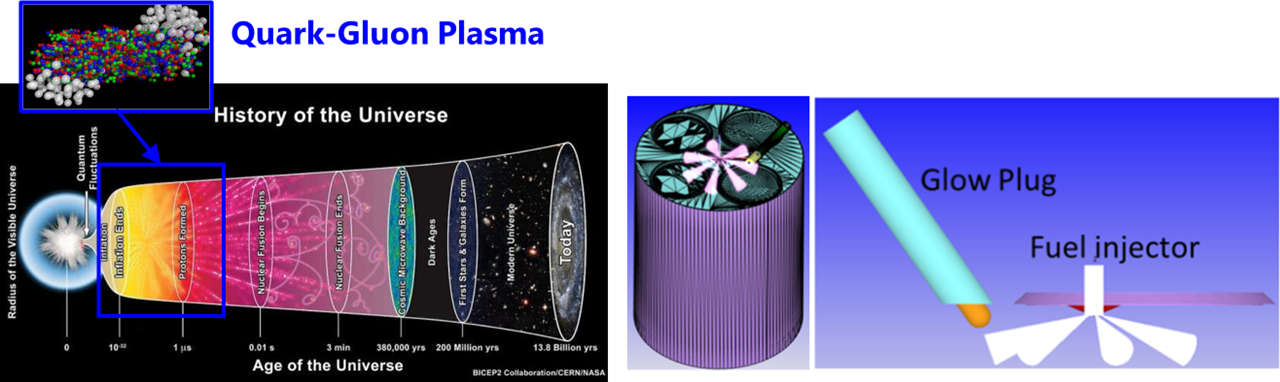
\includegraphics[width=0.80\textwidth]{ProgramsImages/mot.png}
    \caption{(Left) Visualizing the QGP shortly after the Big Bang \cite{qgp}, which became the building blocks of matter in the Universe. \; (Right) A schematic of the UAV metal engine: fuel is injected at seven nozzles, then ignited via a glow plug. \vspace{-3ex}}
    \label{fig:mot}
\end{figure}

These challenges necessitate two crucial ingredients to facilitate scientific discovery: cost-efficiency and confidence. The first, \textit{cost-efficiency}, refers to statistical methods which aim to maximize model performance given a limited cost (e.g., computational) budget. For the earlier nuclear physics problem, a cost-efficient method strives to provide an accurate solution to the inverse problem given a limited computational budget (and thus limited simulation runs). The second, \textit{confidence}, refers to methods which provide a reliable and estimable measure (or quantification) of model error. Such confidence is essential for verifiable scientific discovery: it provides a quantification of uncertainty for findings, thus protecting against spurious findings. This further allows for theoretically sound stopping rules which guarantees model performance, which is particularly crucial for the current cost-constrained setting. For our nuclear physics problem, a confident method yields a measure of uncertainty for the inverse problem, which can be used to guide the amount of simulation runs needed to ensure a desired error tolerance.

Both of the above bottlenecks can be alleviated via a careful integration of novel \textit{sampling} algorithms within the statistical learning framework. Here, ``sampling'' refers to the drawing of representative samples $\bT_1, \dots, \bT_n$ from a (potentially) complex probability distribution $\Pi$, \marginpar{\FJHNote{Is there any conflict between $\Pi$ and $F$ for distribution function?}} and the use of such samples for scientific inference and decision-making. For the first bottleneck of \textit{costly} scientific data, a careful sampling design of the input parameters for the expensive simulator can enable accurate and precise scientific inference in reasonable turnaround times. For the second bottleneck of \textit{massive} data, a judicious sampling of such large datasets can allow for timely scientific discovery for useful decision-making. There is, however, much to be done on \textit{cost-efficient} and \textit{confident} sampling algorithms, given the complexities present in modern scientific problems. We will propose a suite of methods, with supporting theory and algorithms, which address this important gap. We first present the prototypical problem of interest, then provide a survey of \textit{low-discrepancy} sampling methods \citep{niederreiter1992random}, which we extend for our suite of methods.

\subsection{Background.}
\label{sec:background}

We first provide a brief background on the prototypical problem we aim to address, then discuss existing literature and its limitations for our motivating applications. 

\subsubsection{Prototypical Problem.}

Consider the estimation of the \emph{expectation of a random variable} $Y$ whose distribution is some complicated function, $g$, of a random vector $\bT$ with known distribution:
\vspace{-3ex}
\begin{subequations} \label{eq:prototype}
\begin{equation}
\mu := \bbE(Y) = \bbE[g(\bT)] = \, ?
\end{equation}
This arises in many practical problems, e.g., in our \UAV application, $\bT$ may represent uncertainties in engine operating conditions, $g(\bt)$ may denote the engine thrust at operating conditions $\bt$, and we wish to learn the expected engine thrust $\mathbb{E}[g(\bT)]$ under uncertain conditions.

In turn, we define a transformation, $\bPsi$, of a \emph{standard uniform} random vector, $\bX$, into $\bT$, so that we may also write $Y$ as a function, $f$, of $\bX$:
\begin{gather} 
    \label{eq:vartrans}
    \bT = \bPsi(\bX), \qquad f(\bx) = g(\bPsi(\bx)) \abs{\partial \bPsi(\bx)/\partial \bx}, \qquad \bX \sim \calu[0,1]^d, \\
     \mu = \bbE[f(\bX)] = \int_{\cube} f(\bx) \, \dif \bx = \, ?.
\end{gather}
\end{subequations}
This expectation can also be thought of as a \emph{multivariate integration} problem. We need to write $Y = f(\bX)$ because the \LD sequences described later that we intend to use to approximate $\mu$ mimic uniform random vectors. 

% \footnote{We use $\varrho$ to designate the probability density because $f$ is typically used for the integrand in the numerical integration literature.}

Besides the integral problem in \cref{eq:prototype},  it is often useful to know the \emph{distribution}, $F$, \emph{density}, $\varrho$, and/or \emph{quantile} function, $Q$, of $Y$, i.e.,
\begin{subequations} 
\small \label{eq:distdensquant}
	\begin{gather}
		F(y) := \bbP(Y \le y) = \bbP[f(\bX) \le y] = \int_{[0,1]^d} \bbone_{(-\infty,y]}(f(\bx)) \, \dif \bx, \quad \varrho(y) := F'(y), \quad Q(p) := F^{-1}(p).
	\end{gather}
\end{subequations}
In the \UAV problem, we may wish to learn the distribution of engine thrust $Y$ under uncertain operating conditions---these are the primary quantities of interest when designing for robust engines. We will address these problems in \cref{sec:distdensquant} in the context of our motivating applications.

In practice, the population mean or multivariate integral, $\mu$, often cannot be evaluated by analytic means, but it may be estimated by the sample mean, $\hmu_n$, i.e., 
\begin{equation} \label{eq:mean}
    \mu \approx
\hmu_n := \frac 1n \sum_{i=1}^n Y_i = \frac 1n \sum_{i=1}^n f(\bX_i), \qquad Y_i = f(\bX_i).
\end{equation}
Given an error tolerance, $\varepsilon$, we want to choose samples, $\bX_1, \ldots, \bX_n$, to mimic $\calu[0,1]^d$ and satisfy
\begin{equation} \label{eq:error_crit}
	\abs{\mu -\hmu_n} \le \varepsilon \qquad \text{with high confidence}.
\end{equation}

\subsubsection{Low Discrepancy Sampling.}\label{sec:lowdiscrep}

%\cmtS{Fred / Yuhan: pls shorten \& focus after my writing above.} 
Choosing $\bX_1, \bX_2, \ldots$, for evaluating the sample mean in \eqref{eq:mean} to be \hypertarget{IIDlink}{\emph{independent and identically distributed}} (\IID) yields a root mean square error of $\sqrt{\bbE[\abs{\mu -\hmu_n}^2]} = \std(f(\bX))n^{-1/2}$, which is independent of the dimension, $d$, but slowly vanishing as $n \to \infty$. The computational cost to satisfy the error tolerance \eqref{eq:error_crit} is $\Order(\varepsilon^{-2})$. Tensor product generalizations of one-dimensional numerical integration rules using grid sampling give errors of $\abs{\mu -\hmu_n} = \Order(n^{-r/d})$ and a computational cost of $\Order(\varepsilon^{-d/r})$, where $r$ is limited by both the sophistication of the rule and the smoothness of the integrand, $f$.  Such rules may be suited for small $d$, but they are inefficient for the larger $d$ that occurs in our applications of interest.

A superior approach that combines the intentional structure of a grid with the essentially dimensionless error bound of \IID sampling is \LD  sampling, $\bX_1, \bX_2,  \ldots \LDSim \calu[0,1]^d$, which has an error bound of \cite{Nie92,Hic99a}
\begin{equation} \label{eq:KH}
 \abs{\mu - \hmu_n} \le D(\{\bX_i\}_{i=1}^n) \norm[\calf]{f - \mu}.
\end{equation}
The discrepancy,  $D(\{\bX_i\}_{i=1}^n)$, corresponds to the norm of the cubature error functional \cite{Hic97a} for the function space $\calf$.  The discrepancy is also a measure of how close the empirical distribution (which assigns equal probability to each point) is to the uniform distribution. 
The discrepancy is typically $\Order(n^{-1 + \delta})$, where $\delta$ is arbitrarily small and positive. This faster convergence rate translates into a computational cost of $\Order(\varepsilon^{-1-\delta})$ to satisfy error criterion \eqref{eq:error_crit}, under mild smoothness conditions on $f$.  The semi-norm $\norm[\calf]{\cdot - \mu}$ is called the \emph{variation} and is a measure of function roughness. 

\begin{wrapfigure}{r}{0.3\textwidth}
	\centering
	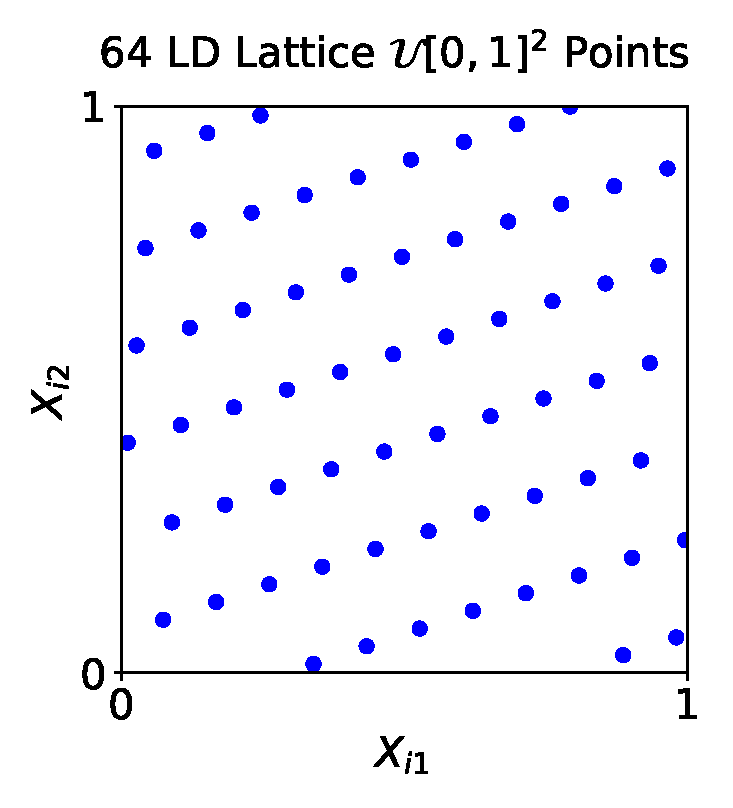
\includegraphics[width = 0.3\textwidth]{ProgramsImages/lattice_scatter.eps}
	\caption{LD lattice points, which have fewer gaps and clusters of points than either the IID or grid points. \label{fig:iid_vs_ld}
 \vspace{-3ex}}
\end{wrapfigure}

Popular \LD sampling schemes include lattices \cite{Nie92,SloJoe94,DicEtal22a} and digital nets \cite{Nie92,DicPil10a}. \cref{fig:iid_vs_ld} displays $n=64$ \LD lattice points intended to mimic $\calu[0,1]^2$.  A two-dimensional grid of $64$ points would only have $8$ different values in each coordinate direction, whereas the \LD sample covers $64$ different values in each coordinate direction. Such schemes are available in many softwares, including 
BRODA \cite{BRODA20a}, 
CUBA \cite{CUBA}
\MATLAB \cite{MAT9.9}, 
\NAG \cite{NAG27}, 
PyTorch \cite{paszke2019pytorch}, 
SciPy \cite{virtanen2020scipy}, 
TensorFlow \cite{tfqf2021a}, 
and uncertainty quantification libraries such as 
Dakota \cite{DakotaUsersManual}, 
MUQ \cite{MUQ}, 
UQLab \cite{UQLab2014}, and 
UQTk \cite{DebEtal04,UQTk}.  Efforts to identify better \LD sequence generators include LatNet Builder \cite{LatNet} and the Magic Point Shop \cite{Nuy17a}. 

PI \FH, co-PI \YD, \SCTC, \MM, \JR, %\cmtS{not defined}, 
\AS and collaborators have developed more comprehensive \QMC libraries, GAIL \cite{ChoEtal21a} for \MATLAB and \hypertarget{QMCPylink}{QMCPy} \cite{QMCPy2020a} for Python.  These libraries include the stopping criteria mentioned below, as well as flexible variable transformations of the form \eqref{eq:vartrans}.  Our recent effort is focused on \QMCPy, and includes an active repository \cite{QMCPy2020a}, documentation \cite{QMCPyDocs}, a tutorial \cite{QMCPyTutMovie2020}, and a blog \cite{QMCBlog}.

\subsubsection{Error Bounds and Stopping Criteria.} \label{sec:stopcrit}
Algorithms based on efficient \LD sampling are commonly called \hypertarget{QMClink}{\emph{quasi-Monte Carlo}} (\QMC) algorithms. To construct a \QMC algorithm, one needs not only an \LD sequence but also \textit{reliable} and \textit{practical} bounds on the error $\abs{\mu - \hmu_n}$ which are based on the function data, $f(\bX_1), f(\bX_2), \ldots$.  Such \textit{data-based} error bounds inform the stopping criteria, which guide the determination of sample size $n$ needed to satisfy the error tolerance \eqref{eq:error_crit}. One approach is to use $N$ different randomizations of a single \LD sequence to compute $N$ sample means, and then estimate the error of the grand sample mean, $\hmu_{nN} = (\hmu_n^{(1)} +  \cdots \hmu_n^{(N)})/N$, via, e.g., bootstrapping. But this would be too costly for our motivating applications since it requires $nN$ evaluations of the expensive function $f$ (see first bottleneck in \cref{sec:motiv}).

 % or the variance of these $N$ sample means

PI \FH and his collaborators have developed two kinds of theoretically justified stopping criteria for \LD sampling based on the Fourier coefficients of the data $f(\bX_1), f(\bX_2), \ldots$.  The first kind determines a bound on $\abs{\mu-\mu_n}$ by inferring the roughness of $f$ from the decay of the discrete Fourier coefficients \cite{HicJim16a,JimHic16a,HicEtal17a}.  The second kind uses  Bayesian credible intervals for $\abs{\mu-\mu_n}$ assuming that $f$ is an instance of a Gaussian process whose hyperparameters are tuned by the function data \cite{HicJag18b,RatHic19a,JagHic22a}. The cost of bounding the error $\abs{\mu-\mu_n}$ is only $\Order(n \log(n))$ for both kinds of stopping criteria.  This can be achieved for the Bayesian approach by choosing covariance kernels that match the \LD sampling schemes, and thus avoiding the typical $\Order(n^3)$ cost.


\subsection{Limitations of Existing Methodology and Software.} \label{sec:limit}

There are, however, fundamental limitations which prevent the effective use of existing methods for tackling the complexities in our applications. These limitations, detailed below, are gaps which we will address in our proposal.

% \begin{enumerate}[label=Limitation \arabic{enumi}, leftmargin=*]
% \item
\subsubsection*{\textup{Limitation 1:}} \hypertarget{LimOneLink}{\textit{Expensive Bayesian Sampling}.} Bayesian inference \citep{gelman1995bayesian} is a popular statistical framework for tackling scientific problems. Here, parameters of interest are sampled from a ``posterior'' probability distribution $\varrho$, which captures both the the prior belief of the modeler and evidence from the collected data. In practical problems, the posterior distribution $\Pi$ is often highly complex and available only in proportional form. This is further complicated by the \textit{costly} nature of each posterior evaluation (see first bottleneck in \cref{sec:motiv}). For example, \textit{each} evaluation of $\Pi$ \marginpar{\FJHNote{$\Pi$ or likelihood?}} in our heavy-ion physics inverse problem requires thousands of CPU hours \cite{everett2021multisystem}. Existing work on \LD sampling, however, focuses largely on the setting of uniform $\Pi$ (a literature review is provided later).  We develop in \cref{sec:bayes} a novel cost-efficient \LD posterior sampling method which addresses this need, with applications to our heavy-ion physics application and broader scientific problems.
% \end{enumerate}

\subsubsection*{\textup{Limitation 2:}} \hypertarget{LimTwoLink}{\textit{Multifidelity Modeling}.} 
For many scientific computing problems, the random variable of interest $Y_\fidparam = f_\fidparam(\bX_\fidparam)$ is parameterized by a \emph{fidelity} parameter $\fidparam$, and the desired quantity of interest is the limiting mean $\mu_\infty = \lim_{\fidparam \to \fidparam_\infty} \bbE(Y_\fidparam)$. In our heavy-ion application, $f_\fidparam(\bX_\fidparam)$ may represent a observable simulated from a complex partial differential equation (PDE) system modeling the heavy-ion collision, with random coefficients $\bX_\fidparam$ representing uncertainties in simulation inputs, and mesh-size parameters $\fidparam$ controlling simulator fidelity. As fidelity increases, the cost of sampling %\cmtS{sampling?} 
$Y_\fidparam$ also increases (as each evaluation $f_\fidparam$ becomes more expensive), and thus the evaluation many high fidelity $Y_{\fidparam,i}$ to approximate $\mu_\infty$ can be prohibitively costly.

Multifidelity (also known as multi-level or multi-index) methods \cite{Hei01a, Gil15a, HajNobTem16a} choose a sequence of fidelity parameters, $\fidparam_1, \fidparam_2, \ldots$, and write the  desired quantity as a telescoping sum: 
\[
\mu = \mu_\infty = (\mu_{\fidparam_1} - \mu_{\fidparam_0}) + (\mu_{\fidparam_2} - \mu_{\fidparam_1}) + \cdots +
(\mu_{\fidparam_L} - \mu_{\fidparam_{L-1}}) + (\mu_{\infty} - \mu_{\fidparam_{L}}), \qquad \mu_{\fidparam_0} = 0.
\]
The sequence of fidelity parameters is chosen so that the cost of evaluating $f_{\fidparam_l}(\bX_{\fidparam_l})$  increases with $l$ (greater fidelity), but the sample size required to estimate $\mu_{\fidparam_l} - \mu_{\fidparam_{l-1}}$ accurately decreases with $l$. The term  $\mu_{\infty} - \mu_{\fidparam_{L}}$ is approximated by zero. Substantial cost-efficiency is gained by using many cheap samples to approximate the low fidelity terms and relatively fewer expensive samples to compute the high fidelity terms. While there is a rich literature on multifidelity methods (including recent work by PIs \SM and \FH, which we discuss later), there has been little work on developing measures of confidence or stopping criteria (see \cref{sec:stopcrit}) for such multifidelity methods. Such stopping criteria are important for our heavy-ion application, allowing for confident scientific inference with minimal experimental costs. We will addressed such limitations in \cref{sec:stopmulti}.

\subsubsection*{\textup{Limitation 3:}} \hypertarget{LimThreeLink}{\textit{Big Data Analysis}.} Given sophisticated computing technology, scientific simulators typically output massive datasets with complex forms, and the efficient use of such data for scientific discovery is paramount. One solution is to take a small representative \textit{subsample} of the big data, and use this for efficient model training. The careful selection of this subsample is critical for timely decisions. Machine learning algorithms often makes use of stochastic gradient descent \cite{Bot2010,srivastava2014dropout}, which takes a new \textit{random} subsample of the big data at each gradient update; such random subsampling, however, may be practically and theoretically inefficient given a computational constraint (more on this later). There has been recent work on extending \LD ideas for big data subsampling (discussed later), but such methods typically do not perform well or have sound theoretical guarantees for complex learning models (e.g., neural networks) which are desired with massive training data. To address this, we propose in \cref{sec:bigdata} a new \LD subsampling method, which provides provably improved \LD big data subsampling for a broader class of learning models.

\subsubsection*{\textup{Limitation 4:}} \hypertarget{LimFourLink}{\textit{Distribution, Density, and Quantile Estimation}.} 
In many problems, practitioners wish to estimate not only the mean of $Y = g(\bT)$, but also its distribution, density or quantile (as defined in \cref{eq:distdensquant}). This is the case in our \UAV problem: aerospace engineers wish to estimate not only the expected engine thrust $E(Y)$ under uncertain operating conditions $\bT$, but also characterize its full distribution for designing robust engines. The error analysis for such problems, especially for \LD sequences, is underdeveloped in the literature, and the rigorous, data-based stopping criteria are non-existent. We address this limitation in  \cref{sec:distdensquant}.

% In Bayesian inference one may want to compute the marginal distributions of a random vector $\bY = \bg(\bT) = \bff(\bX)$.

% \subsubsection*{\textup{Limitation 5:}} \hypertarget{LimFiveLink}{\textit{Automatic Variable Transformations}.}  \cmtS{move to Lim 2?}
% There are often multiple possible transformation $\bPsi$ that map to $\bT$ from a standard uniform random variable $\bX$ as in \eqref{eq:vartrans}.  For example, mapping $\bX \sim \calu[0,1]^d$ to $\bT \sim \caln(\bzero,\mSigma)$  involves choosing one of infinitely many possible square roots of the covariance matrix, $\mSigma$, (for $d>1$).  Choosing transformation $\bPsi$ to give an integrand $f$ with small roughness, i.e., small variation, $\norm[\calf]{f - \mu}$ is nontrivial and ideally should be based on function data. This may be addressed by adaptive importance sampling and/or control variates. We address this limitation in \cref{sec:imp}.

\subsubsection*{\textup{Limitation 5:}} \hypertarget{LimSixLink}{\textit{Software Quality}.} 
\QMC software implemented by non-experts may be flawed.  \FH and \MM found  that randomized \PyTorch Sobol' points fell on the boundaries of $[0,1]^d$, when they never should \cite{PyTorchFirstPt2020a} due to a lack of double precision.  \hypertarget{LlAJRlink}{Llu\'is Antoni Jim\'enez Rugama} (\LlAJR), a former PhD student of \FH,  alerted  that \MATLAB's Sobol' sequence scrambling was incorrect; \MATLAB later corrected this error.  After a vigorous discussion on the \PyTorch \cite{PyTorchFirstPt2020a} and  \SciPy  \cite{scipySobol2020a} issues sites, \AO, \FH, and other \QMC researchers convinced the developers not to omit the first Sobol' point and to randomize by default. \AO explained why this is crucial~\cite{owen2020dropping}.   The need for a vigilant \QMC software community is addressed in  \cref{sec:provingground}. Further, solving complex problems well and efficiently often requires multiple software libraries.  For example, in uncertainty quantification, one integrand, $f(\bX_i)$, may be the output from a PDE library.  Not all libraries connect well, nor are there yet standards in the QMC software community on how to pass information from one library to the next. We address this issue in \cref{sec:provingground}.



% \subsection{Proposed Framework} How does our proposed framework tackle the aforementioned motivating limitations? What are specific objectives we aim to address? Should highlight \QMCPy as a vessel for dissemination of our product to the broader scientific community. Should also tout our credentials in software development and collaborative experience with cutting-edge scientific \& big data applications. \cmtS{add workflow figure going from applications to tasks.}

% \subsection{Scientific Impact}
% \label{sec:sci}
% Outline the envisioned applications \& impact for the proposed framework: (Add visualization of problem)
% \begin{itemize}
% \item Physics discovery for high energy physics (Simon, with the JETSCAPE collaboration): surrogate modeling \& Bayesian inference for heavy-ion collisions
% \item Real-time control of \UAVs (Simon, with UMinn collaborators): real-time control via virtual engines for unmanned aerial vehicles (big data, emulation)
% \item Bayesian optimization (Fred, Mike McCourt). Applications in food science: Simon will ping a collaborator (former student) in industry.
% \item \cmtS{Fred: random coefficients in PDE, for engineering applications.}
% \end{itemize}
% Should also talk about broader impacts of an open-source software and its impact on scientific progress. Can reiterate some of onon 4 here in the context of addressing aforementioned applications and problems.

% \subsection{}

% The theoretical and methodological questions addressed by this project will include 
% \begin{enumerate}[i)]
% \item Reliable adaptive importance for QMC cubature (\cref{sec:imp});
% \item $\Order(n^{-3/2})$ convergence with scrambled nets for integrals over $\reals^d$ (\cref{sec:threehalves});
% \item Stopping criteria for higher-order digital net (\cref{sec:HONstop}) and multilevel QMC cubatures (\cref{sec:stopML});
% \item Multilevel QMC function approximation (\cref{sec:MLAppx});
% \item \LD subsampling for big data analytics to decrease computational cost (\cref{sec:bigdata}); and
% \item \LD posterior sampling methods for expensive Bayesian modeling problems (\cref{sec:bayes}).
% \end{enumerate}

% \cmtS{to modify, move later into \SEC 1? and have this has a one-paragraph abstract on the overarching framework \& broader impacts?}







%%%%%%%%%%%%%%%%%%%%%%%%%%%%%%%%%%%%%%%%%%%%%%%%%
\section{A Framework for Cost-Efficient and Confident Sampling}
\label{sec:tasks}
%%%%%%%%%%%%%%%%%%%%%%%%%%%%%%%%%%%%%%%%%%%%%%%%%
We now present a suite of novel methods (with supporting theory and algorithms) which extend \LD sampling to the complex settings from our motivating applications. These methods provide a useful toolbox for cost-efficient and confident sampling to accelerate scientific discovery. Figure \ref{fig:workflow} shows the workflow for the four proposed tasks, which directly address the limitations in \cref{sec:limit}.

\begin{figure}[!t]
\centering
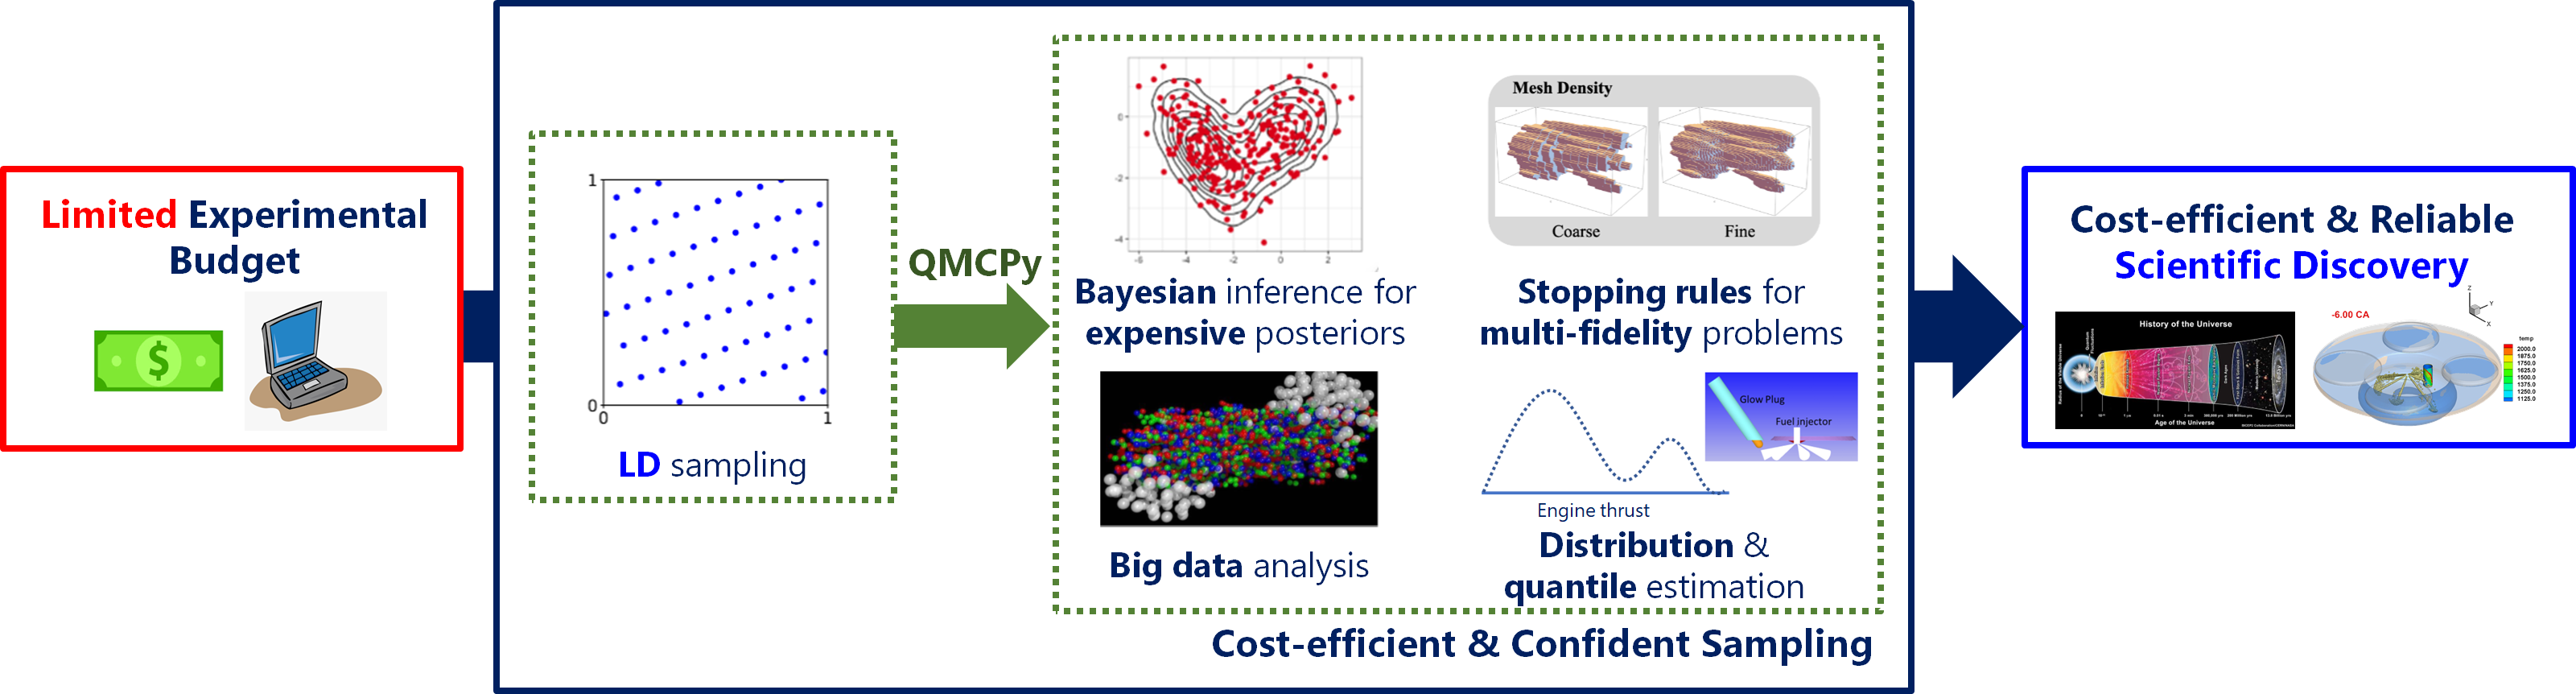
\includegraphics[width=0.9\textwidth]{ProgramsImages/workflow.png}
\caption{Project workflow: given a limited budget, the proposed tasks (\cref{sec:tasks}) extend LD sampling to the complex settings motivated by our applications, providing a toolbox for cost-efficient and reliable scientific discovery. QMCPy (\cref{sec:provingground}) serves as an open-source software package that disseminates our suite of methods to the scientific community.\vspace{-7ex}}
\label{fig:workflow}
\end{figure}

%%%%%%%%%%%%%%%%%%%%%%%%%%%%%%%%%%%%%%%%%%%%%%%%%
\subsection{Bayesian Sampling for Expensive Posteriors} [\SM lead, \FH, \IJi, \TT, \JM{}] \label{sec:bayes}
%%%%%%%%%%%%%%%%%%%%%%%%%%%%%%%%%%%%%%%%%%%%%%%%%

%%%%%%%%%%%%%%%%%%%%%%%%%%%%%%%%%%%%%%%%%%%%%%%%%
\subsubsection{Background and Preliminary Results.}
%%%%%%%%%%%%%%%%%%%%%%%%%%%%%%%%%%%%%%%%%%%%%%%%%
Bayesian methods \cite{gelman1995bayesian} rely on MCMC sampling to explore the posterior distribution $F$, which captures information on model parameters (see PI \SM's work \cite{mak2016regional,huang2022population,mak2021tsec}). However, $F$ can often be \textit{expensive} to evaluate in many scientific computing problems (see \LimOne). This is compounded by the highly correlated nature of traditional MCMC samplers, which reduces the information provided by each sample \citep{link2012thinning}. Existing samplers for such problems thus be prohibitively \textit{costly} \cite{joseph2015sequential}, and an LD posterior sampling method can provide improved Bayesian learning given a computational budget.


% While the QMC Metropolis method by \cite{OweTri05a} speeds up the convergence of samples, it still requires many posterior evaluations. We want method which can provide \LD sampling with limited posterior evaluations here.

One approach for \LD posterior sampling is to minimize the \textit{kernel discrepancy} $D_K(\{\bT_i\}_{i=1}^n, F)$ \cite{Hic99a}, which measures the difference between the empirical distribution of $\{\bT_i\}_{i=1}^n$ and the posterior $F$ via a symmetric positive-definite kernel $K$. This approach, known as \textit{kernel herding} \citep{chen2012super}, has a key limitation: the discrepancy requires an analytic form for the integral $\int K(\bt,\cdot) \, \dif F(\bt)$, which is unattainable for complex posteriors $F$. To address this, \cite{chen2018stein} proposed the ``Steinized'' kernel:
\begin{multline}\label{eq:stein}
K_{\rm ST}(\bt,\bx) = \nabla_\bt \cdot \nabla_\bx K(\bt,\bx) + \nabla_\bt K(\bt,\bx) \cdot \nabla_\bx \log \dif F(\bx)\\
 + \nabla_\bx K(\bt,\bx) \cdot \nabla_\bt  \log \dif F(\bt) + K(\bt,\bx) \nabla_\bt \log \dif F(\bt) \cdot \nabla_\bx \log \dif F(\bx),
\end{multline}
where $\nabla$ and $\nabla \cdot$ are the gradient and divergence operators. With this, $\int K_{\rm ST}(\bt,
\cdot) \, \dif F(\bt)$ evaluates to 0, thus yielding a closed form expression for the \textit{kernel Stein discrepancy} (KSD):
\begin{equation}
    D_K(\{\bT_i\}_{i=1}^n, F) := \sqrt{\frac{1}{n^2}\sum_{i,j=1}^{n}K_{\rm ST}(\bT_i, \bT_j)}, \quad K = K_{\rm ST}.
    \label{eq:ksd}
\end{equation}
\cite{chen2018stein} then employs a sequential optimization of the KSD: the first sample $\bT_1^*$ is taken at the mode of $F$, then subsequent samples $\bT_2^*, \bT_3^*, \cdots$ are obtained by sequentially optimizing the KSD, i.e.:
\begin{equation}
\bT_n^* \leftarrow \argmin_{\bt} \text{KSD}_n(\bt) := \argmin_{\bt} D_K(\{\bT_i^*\}_{i=1}^{n-1} \cup \bt, F), \quad K = K_{\rm ST}, \quad n = 2, 3, \cdots.
\label{eq:ksdopt}
\tag{$\text{ESP}_n$}
\end{equation}
These optimized samples, called \textit{Stein points}, gives improved representation of the posterior $F$ over standard MCMC methods for a fixed sample size $n$.

However, Stein points have a key drawback: they are \textit{not} cost-efficient. When the posterior $F$ is expensive, the optimization of the Stein discrepancy for a \textit{single} sample point will require \textit{many} evaluations of $F$ in the form of its score function $\nabla_\bt \log \dif F(\bt)$. For our heavy-ion application, given a fixed budget of $10^6$ CPU hours, we can afford $10^3$ evaluations of $F$, which translates to only $n \approx 50$ Stein points - this is inadequate for exploration of complex posterior distributions.

We thus propose the following cost-Efficient Stein Points (ESPs). The key idea is the construction of a sequence of carefully constructed Gaussian process (GP) surrogate models \citep{santner2003design} on the expensive objective functions $\text{KSD}_n$. Consider first \eqref{eq:ksdopt} for a given $n$. Suppose the posterior in the form of its score function $\nabla_\bt \log \dif F(\bt)$ has already been at evaluated at $M_{n}$ candidate points $\{\bT_j\}_{j=1}^{M_{n}}$, yielding objective evaluations $\mathcal{D}_n = \{\text{KSD}_n(\bT_j)\}_{j=1}^{M_n}$ via \eqref{eq:ksd}. Under a GP prior on $\text{KSD}_n(\cdot)$, the posterior distribution of $\text{KSD}_n(\bt)$ can be shown to be $\text{KSD}_n(\bt)|\mathcal{D}_n \sim \mathcal{N}\{\mu_n(\bt),\sigma^2_n(\bt)\}$; specific forms for $\mu_n(\bt)$ and $\sigma^2_n(\bt)$ can be found in \cite{santner2003design}. Using this and following the literature on Bayesian optimization (e.g., \cite{jones1998efficient} and work from PI \SM \cite{chen2019hierarchical}), the \textit{expected improvement} in objective $\text{KSD}_n$ from evaluating the posterior at a new point $\bt$ takes the closed-form expression:
\begin{equation}
    \text{EIKSD}_{n}(\bt) = (\text{KSD}_{n,\rm{min}} -  \mu_n(\bt)) \Phi \left(\frac{\text{KSD}_{n, \rm{min}} -  \mu_n(\bt)}{  \sigma_n(\bt)} \right) +  \sigma_n(\bt) \phi \left(\frac{\text{KSD}_{n,\rm{min}} -  \mu_n(\bt)}{  \sigma_n(\bt)}\right),
    \label{eq:ei}
\end{equation}
where $\text{KSD}_{n,\rm{min}}$ is the best observed $\text{KSD}_n$ value. We thus wish to evaluate the expensive posterior at the point that maximizes $\text{EIKSD}_{n}(\bt)$. This procedure, of refitting the GP surrogate and evaluating the posterior at the point of greatest expected improvement, is then iterated until a convergence criterion is met. The evaluated point with smallest $\text{KSD}_n$ is then taken as the next sample $\bT_n^*$ in \eqref{eq:ksdopt}.

\begin{wrapfigure}{r}{0.55\textwidth}    \centering
    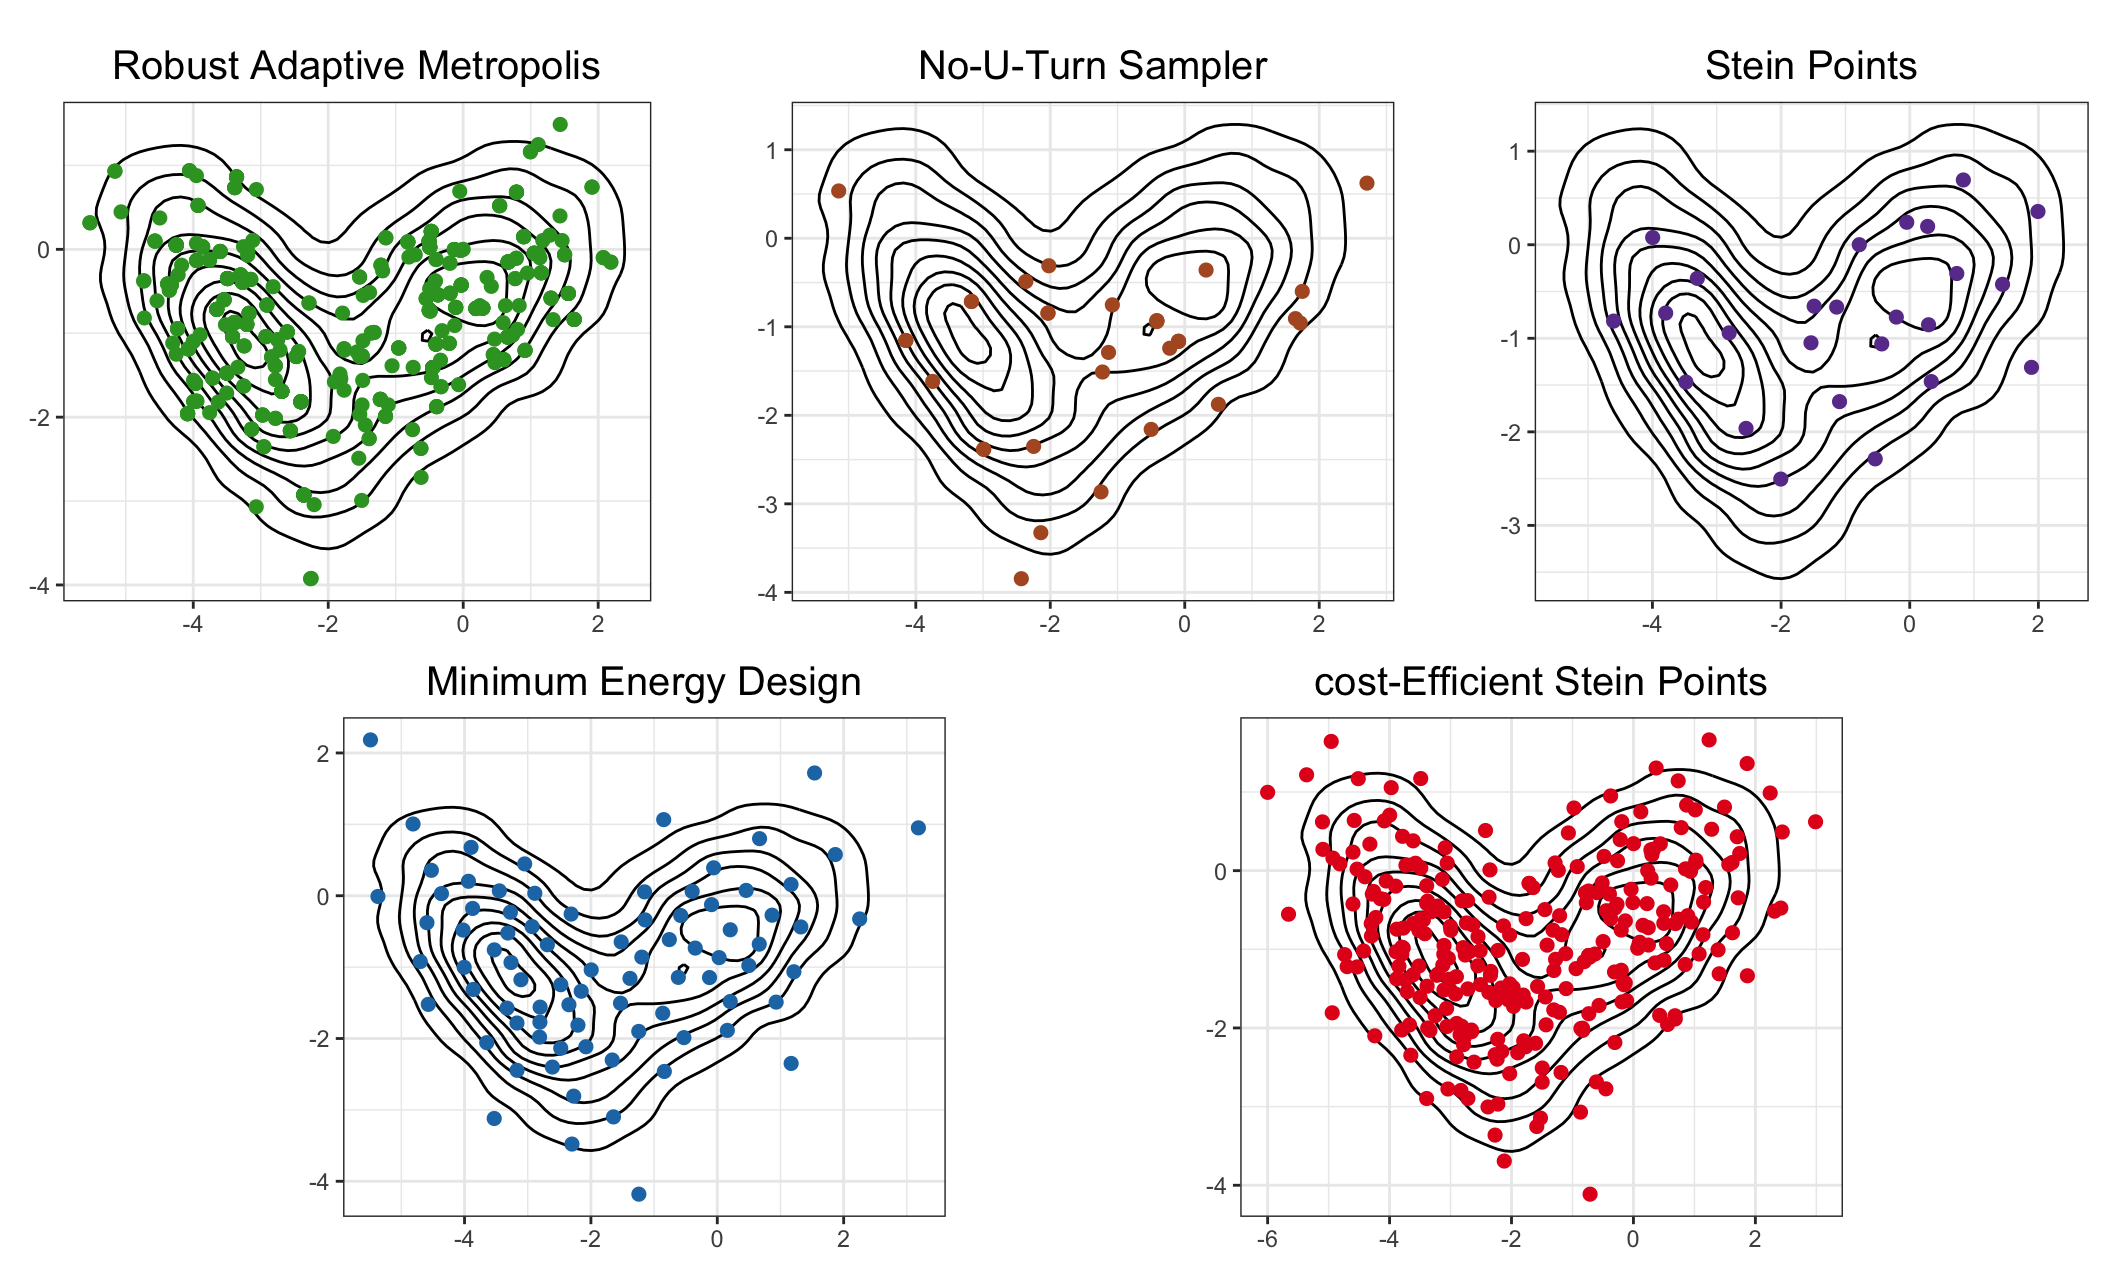
\includegraphics[width=0.55\textwidth]{ProgramsImages/2d2m_corr_500Evals.png}
    \caption{Visualizing the sampled points on a 2D two-mixture normal distribution, using four existing posterior samplers and the proposed ESPs. All samplers are limited to 500 posterior evaluations. \vspace{-3ex}}
    \label{fig:esps}
\end{wrapfigure}
Consider next the \textit{sequence} of optimization problems in \eqref{eq:ksdopt} for ESP sampling. A key observation is that the posterior evaluations used for solving previous problems $\text{ESP}_2, \cdots, \text{ESP}_{n-1}$ can be directly \textit{reused} for the current problem $\text{ESP}_{n}$, since such evaluations translate directly to evaluations of $\text{KSD}_n$ via \eqref{eq:ksd}. Thus, as sample size $n$ increase, this allows for increasingly more data on the objective $\text{KSD}_n$ to generate the $n$-th ESP $\bT^*_n$. This recycling of posterior evaluations enables cost-efficient ESP sampling given a limited computational budget.

To demonstrate the cost-efficiency of ESPs, \cref{fig:esps} compares several state-of-the-art samplers (the robust adaptive Metropolis sampler \citep{vihola2012robust}, the No-U-Turn sampler \citep{hoffman2014no}, Stein points \citep{chen2018stein}, minimum energy designs \citep{joseph2015sequential}) on a 2D two-mixture normal distribution. All samplers are limited to $B=500$ posterior evaluations. We see that, as expected, existing samplers that ignore the expensive nature of posterior evaluations provide a poor approximation of $F$: they either yield a small sample size ($n \approx 50$), or a highly correlated sample chain. ESPs, on the other hand, provide a noticeably larger sample size $n = 287$ with low sample correlation. This improved posterior representation is confirmed via a comparison of marginal statistics or distributional metrics. 








% Despite this, Stein points have a key limitation: they do not provide \textit{inference} for computed posterior quantities. Suppose we estimate the posterior mean $\mu = \mathbb{E}_{\bX\sim F}[g(\bX)]$ with $\hat{\mu}_n = n^{-1}\sum_{i=1}^n g(\bX_i^*)$, where $\{\bX_i^*\}_{i=1}^n$ are the Stein points. With these \textit{deterministic} samples, it is difficult to infer the error $|\mu - \hat{\mu}_n|$, since the deterministic error bounds for Stein points (see \cite{chen2018stein}) contain many constants which cannot be estimated in Bayesian problems. But the quantification of estimate uncertainty is paramount for expensive Bayesian problems: it provides a principled way to assess whether the posterior sample taken is large enough for validating scientific findings.

% We propose a novel \textit{Randomized Stein points} (RSPs) method which addresses this need. This idea is inspired by randomized lattice rules (see \cite{l2002recent}), which randomizes lattices on $[0,1]^d$ by randomly shifting its first point. Here, instead of taking the first sample $\bX_1^*$ at the \textit{mode} of $F$, we select this point  \textit{randomly} from $F$ (e.g., after an initial MCMC burn-in). Subsequent samples $\bX_2^*, \bX_3^*, \cdots$ are then obtained via sequential optimization of $D(\{\bX_i\}_{i=1}^n, F)$, similar to the original Stein points. This random initialization for RSPs allows for probabilistic inference on error $|\mu - \hat{\mu}_n|$. Since the samples $\{\bX_i^*\}_{i=1}^n$ are now \textit{random}, one can now apply probabilistic confidence intervals used for standard MCMC samplers (e.g., \cite{atchade2016markov,rosenthal2017simple}). \cref{fig:rsp} compares the performance of RSPs with two popular MCMC samplers: Random-Walk Metropolis (RWM, \cite{metropolis1953equation}) and the Metropolis-Adjusted Langevin Algorithm (MALA, \cite{roberts1996exponential}), for a simple 1-d mixture normal distribution $F$. The left plot shows the effective sample size (ESS, a measure of sample quality \cite{GelEtal13}) of $n=300$ samples, and the right plot shows the length and coverage ratio of a simple 95\% confidence interval (CI) $\hat{\mu}_n \pm 1.96 \hat{\sigma} / \sqrt{\text{ESS}}$ for the mean of $F$, where $\hat{\sigma}^2$ is the estimated variance of the integrand. We see that RSPs enjoy noticeably improved sample quality (higher ESS), which translates to more precise CIs (smaller CI length) and higher coverage ratios. This suggests the proposed RSPs indeed provide the improved sample efficiency and uncertainty quantification required for expensive Bayesian problems.

% \begin{wrapfigure}{r}{0.45\textwidth}
% 	\centering
% 	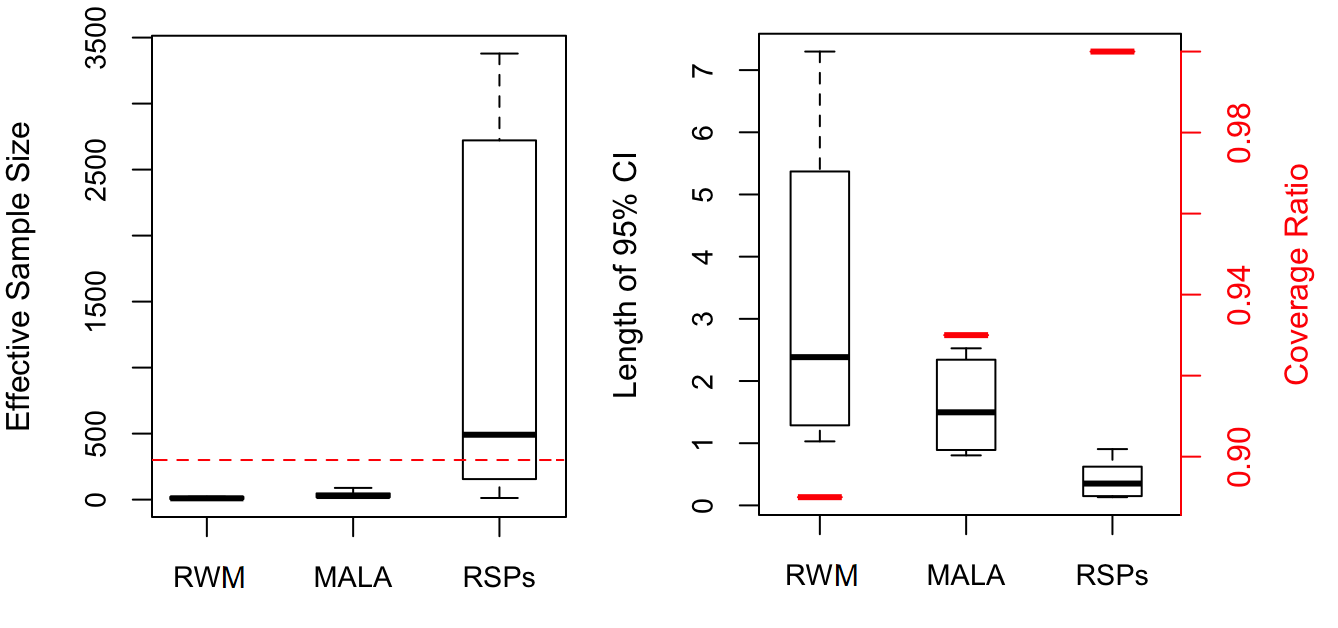
\includegraphics[width = 0.45\textwidth] {ProgramsImages/rsp.png}
% 	\caption{ESS (left) and CI length / coverage ratio (right) for $n=300$ samples using RMW, MALA and RSPs. Boxplots show the distribution of metrics over 100 simulation replications. \label{fig:rsp}}
% 	\vspace{-0.6cm}
% \end{wrapfigure}

% We will tackle the following tasks to develop RSPs for efficient Bayesian learning in \QMCPy.
%%%%%%%%%%%%%%%%%%%%%%%%%%%%%%%%%%%%%%%%%%%%%%%%%
\subsubsection{Theory.} [Years 1--3]
%%%%%%%%%%%%%%%%%%%%%%%%%%%%%%%%%%%%%%%%%%%%%%%%%
Given these promising results, we will investigate key theoretical properties for ESP sampling. A key property to establish is, given an error tolerance $\varepsilon$ for posterior approximation, what is the computational cost (i.e., the number of posterior evaluations $B$) required to achieve such a tolerance with ESPs. This provides a theoretical basis for comparison with existing samplers which ignore evaluation costs. Such rates will require a careful integration of cost complexity results for Monte Carlo \citep{giles2015multilevel} with Bayesian non-parametrics theory \citep{hjort2010bayesian}. We will also explore the cost-efficiency of ESPs using a variety of probabilistic surrogate models, particularly models that can learn embedded low-dimensional structure for high-dimensional approximation, and models that can integrate prior scientific information (see papers by PI \SM \cite{chen2020function,zheng2021online,zhang2022gaussian} and \cite{ji2021graphical,ji2022multi,liyanage2022efficient}).

\subsubsection{Randomization and Central Limit Theorems.} [Years 1--2] In \QMC, the \textit{randomization} of \LD sequences is an important emerging topic, providing a basis for probabilistic inference (e.g., confidence intervals) on integral estimands \citep{dick2013high}. Such randomization is particularly important in this expensive Bayesian setting, where a quantification of estimation uncertainty is desired given limited posterior evaluations. We will develop a randomized implementation of ESPs, where in addition to providing an efficient \LD sampling of the posterior, each marginal sample $\bT_n^*$ is \textit{random} and follows the desired posterior distribution. We will further prove a Central Limit Theorem, which characterizes the asymptotic distribution of integral estimators as $n \rightarrow \infty$. With this, we will develop confidence intervals for the proposed randomized ESPs (following \cite{rosenthal2017simple}), and use this to demonstrate the improved cost-efficiency of ESPs over existing MCMC samplers.


%%%%%%%%%%%%%%%%%%%%%%%%%%%%%%%%%%%%%%%%%%%%%%%%%
\subsubsection{Implementation and Application.}
We will demonstrate the usefulness of ESPs in a wide range of modern scientific problems involving expensive Bayesian inference. This includes our motivating heavy-ion application (see \cref{sec:motiv}), where the Bayesian inference of plasma properties from particle colliders requires costly forward runs (thousands of CPU hours) for each evaluation of the posterior. PI \SM has worked extensively in this area (see \cite{everett2021multisystem,everett2021phenomenological,everett2022role,ehlers2022bayesian,fan2022multi,liyanage2022efficient,kumar2022inclusive}) as a member of the JETSCAPE collaboration (discussed later in \cref{sec:jetscape}). We will further explore broader applications of ESPs in Bayesian sensor imaging, rocket engine design and astrophysics, for which the PIs have close ongoing collaborations. The proposed algorithms will be implemented on our open-source package \QMCPy (discussed later in \cref{sec:provingground}).


% \SMNote{expand on novel developments} \textit{We will implement Stein points} in \QMCPy. PI \SM has worked on a variety of complex Bayesian modeling problems, from climatology \cite{mak2016regional} to aerospace engineering \cite{mak2018efficient,chang2019kernel,yeh2018common}, and we will explore the effectiveness of Stein points for such problems. We will also explore further extensions of Stein points for approximate Bayesian computation, a popular class of Bayesian methods for population genetics and epidemiology.
%%%%%%%%%%%%%%%%%%%%%%%%%%%%%%%%%%%%%%%%%%%%%%%%%
\subsection{Adaptive Multifidelity Algorithms} [\FH lead, \SCTC, \YD, \MM, \PR, \CH, \AO, \AS{}] \label{sec:performance}
%%%%%%%%%%%%%%%%%%%%%%%%%%%%%%%%%%%%%%%%%%%%%%%%%

\subsubsection{Motivation.} A common uncertainty quantification problem in the physical sciences involves the estimation of $\mu = \bbE(Y)$, where $Y=f(\bX)$ and $f$ can only be approximated by $f_\fidparam$, with $\fidparam$ denoting the fidelity of the approximation. In geophysics, $f$ may be the solution of a (partial) differential equation modeling fluid flow, whose boundary conditions are given by a random spatial field, and $\fidparam$ may denote the mesh size of the numerical solver and the discretization of the random field. In our heavy-ion application, $f$ may be the exact solution of an particle collision observable from a complex physics model with uncertain plasma properties $\bX$ as inputs, and $\fidparam$ may capture the spatial and temporal mesh size of the simulator (see work on this by PI \SM \cite{ji2021graphical,ji2022multi,liyanage2022efficient}).

As mentioned in \cref{sec:limit}, approximating the true solution, by a single high fidelity expectation can be prohibitively costly. Rather, multifidelity methods \cite{Hei01a, Gil15a, HajNobTem16a}---an active research area---consider a sequence of problems, $\{\mu_l =\bbE[f_{\fidparam_l}(\bX_{\fidparam_l})] \}_{l=0}^L$, where the fidelity increases with $l$ as does the computational cost of evaluating an instance $f_{\fidparam_l}(\bX_{\fidparam_l,i})$.  One can efficiently approximate $\mu$ by using more cheap samples to approximate $\mu_l - \mu_{l-1}$ for small $l$ and fewer  expensive samples to approximate $\mu_l - \mu_{l-1}$ for large $l$. There has been recent work (see \cite{giles2008multilevel, giles2015multilevel}, including recent work by PI \SM \cite{sung2022stacking}) which show that, under mild conditions on the cost function of the simulator $f_{\fidparam}$ and its convergence rates, multifidelity methods can provide noticeably more accurate and confident estimates over single-fidelity approaches, given a cost budget $B$. 

Despite this, there has been little work on stopping criteria for multifidelity sampling methods (see \LimTwo). This is crucial for scientific discovery; in our heavy-ion application, such criteria provide physicists with a confident quantification of uncertainty given a computational budget, or equivalently, a confident estimate of budget required to achieve a desired precision on findings. We propose below two novel directions which address this in a cost-efficient manner.

\subsubsection{Extending Stopping Rules to Multifidelity Problems.}\label{sec:stopmulti} [Years 1-2]
Adaptive algorithms for these multifidelity problems use ad hoc stopping criteria.  We propose to develop  rigorous stopping criteria like those described in \cref{sec:stopcrit}.  PI \FH, \AS,  \JR, and collaborators have  developed stopping criteria for functions of several expectations, $C(\bmu)$, \cite{HicEtal17a, JagSor23a}.  For example, Bayesian posterior means, \cite{GelEtal13}, can be written as the ratio of two  expectations, $C(\bmu) = \mu_2/\mu_1$.  Sensitivity indices \cite{Sob01,Sal02a,SalEtal08a} also involve the  computation of more than one expectation.  However, in both these cases, the underlying random vector, $\bX$, is the same for all expectations, $\mu_1, \mu_2, \dots$, and only the functions $f_l$ defining the expectations are different.

For multifidelity problems each $\mu_l$ depends on a different $\bX_{\fidparam_l} \sim \calu[0,1]^{d_l}$ with a different $d_l$.   Thus, adaptive algorithms need to manage \LD sequences of different dimensions as well as different sample sizes.  Adaptive decisions must be made on whether to devote more effort to sampling the low or high fidelity terms.  The wealth of literature on multifidelity methods and our experience on developing rigorous stopping criteria for single fidelity problems gives us confidence in success.

% \subsubsection{Variance/Variation Reduction Through Importance Sampling} \label{sec:imp} 
% %%%%%%%%%%%%%%%%%%%%%%%%%%%%%%%%%%%%%%%%%%%%%%%%%
% [Years 2--3]  The discrepancy \eqref{eq:KH} measures the difference between the empirical distribution of the sample points and the uniform distribution.  In many cases, the original expectation problem is in terms of a nonuniform random variable, $\bT$, and a variable transformation, as in \eqref{eq:vartrans}, must be performed to obtain an integral over $[0,1]^d$.  Choosing the transformation $\bPsi$ is equivalent to performing importance sampling.   

% Let's denote the result of this variable transformation as $f_\bPsi$ to show the $\bPsi$ dependence, since $\bPsi$ is non-unique.  The Koksma-Hlawka inequality, \eqref{eq:KH}, tells us to choose $\bPsi$ to make the variation, $\norm[\calf]{f_{\bPsi} - \mu}$, small.  For randomized QMC we want to make the variance of $\hmu_n$ small.  Intuitively, variance/variation reduction is making $f_{\bPsi}$ as flat as possible. 

% We will \emph{implement adaptive importance sampling}, drawing on the work of  
% \AO \cite{owen2000safe} for safe importance sampling, the  annealed importance sampler \cite{neal2001annealed}, and the bridge sampler \cite{gelman1998simulating}.  Recent work includes \cite{mueller2019neural}, which uses deep neural networks for importance sampling in image rendering.  In \cite{huling2020energy}, PI \SM extends importance sampling for covariate balancing in causal inference.  \FH's PhD student, \KZ, has shown how importance sampling with \QMC can beat MCMC in simple Bayesian inference problems \cite{Zha21a}.  We will determine \emph{theoretically and empirically} under what conditions adaptive importance sampling makes \emph{significant improvement in computation times.}

\subsubsection{Implementation and Application.} We will demonstrate the effectiveness of the above developments for confident sampling in a broad spectrum of scientific problems involving multifidelity modeling. This includes our motivating heavy-ion application (\cref{sec:motiv}), where the simulators for particle collisions have multiple fidelity parameters involving spatial meshes and time-steps at different stages (see PI \SM's papers \cite{ji2021graphical,ji2022multi}). We will further explore broader applications in geophysical applications, which the PIs have close ongoing collaborations (see \cite{yuchi2021bayesian}). The proposed algorithms will be implemented and fully documented in \QMCPy (see \cref{sec:provingground})



%%%%%%%%%%%%%%%%%%%%%%%%%%%%%%%%%%%%%%%%%%%%%%%%%
\subsection{Big Data Subsampling} [\SM lead, \AO, \IJi, \KL{}] \label{sec:bigdata}
%%%%%%%%%%%%%%%%%%%%%%%%%%%%%%%%%%%%%%%%%%%%%%%%%

%%%%%%%%%%%%%%%%%%%%%%%%%%%%%%%%%%%%%%%%%%%%%%%%%
\subsubsection{Motivation and Preliminary Results.} 
%%%%%%%%%%%%%%%%%%%%%%%%%%%%%%%%%%%%%%%%%%%%%%%%%
Big data is ubiquitous with advances in technology and computing. In our \UAV application, the output of the numerical simulator can require terabytes of storage (see \cref{sec:background}). A key challenge is that learning algorithms need to be \textit{scalable} to extract useful information from such data for \textit{real-time} decisions, e.g., real-time engine control for \UAV flight. One strategy is to iteratively train the model on small batches of the data, typically sampled uniformly at random. This \textit{subsampling} scales up state-of-the-art machine learning algorithms, such as stochastic gradient descent (SGD, \cite{Bot2010}) and stochastic gradient boosting \cite{friedman2002stochastic}.

\sloppypar Consider SGD, which minimizes the loss $L(\theta;\mathcal{T}) = N^{-1} \sum_{m=1}^N l(\theta;\bT_m)$ over model parameters $\theta \in \mathbb{R}^q$, where $\mathcal{T} = \{\bT_m\}_{m=1}^N \subset \mathbb{R}^d$ is the large training data. Standard gradient descent \cite{nocedal2006numerical} is impractical here, since they require evaluation of the full gradient $N^{-1} \sum_{m=1}^N \nabla_\theta l(\theta;\bT_m)$, which is very expensive with $N$ large. Mini-batch SGD \cite{Bot2010} approximates this via a subsample $\mathcal{T}_{s}^{[l]} \subset \mathcal{T}$ of size $n \ll N$, taken \IID and uniformly from $\mathcal{T}$. The descent steps are iterated until convergence:
\begin{equation}\label{eq:sgdopt}
\theta^{[l+1]} \leftarrow \theta^{[l]} - \eta \Biggl( \frac{1}{n} \sum_{\bT \in \mathcal{T}_{s}^{[l]}} l(\theta;\bT)\Biggr) , \quad l = 1, 2, \ldots,
\end{equation}
where $\eta$ is the gradient descent step size. Mini-batch SGD is widely used for scalable training of neural networks and deep learning models with big data \citep{srivastava2014dropout}.

Mini-batch SGD, however, has a key limitation. Since gradients are estimated by \textit{random} subsampling, the solution sequence $(\theta^{[l]})_{l=1}^\infty$ converges to a \textit{noise ball} of radius $\mathcal{O}(n^{-1})$ around the global optimum $\theta^*$. For small subsample sizes $n$ (as necessitated from our cost-constrained setting), SGD can thus return estimates \textit{very far} from  $\theta^*$. Our solution is to choose an \LD dataset that well-represents the big data $\mathcal{X}$. This is known as ``data squashing'' (termed by \AO in \cite{owen2003data}), and encompasses work on leverage-score subsampling \cite{ma2015statistical}, coresets \cite{chan2006faster,bachem2017practical, huggins2016coresets}, and work by PI \SM \cite{mak2018support,mak2018minimax,mak2017projected,krishna2019distributional}. \LD data squashing for SGD is a timely problem, but largely unaddressed in the literature (see \LimThree).
% Existing methods, however, do not apply directly for the problem of data squashing for SGD optimization.

We propose a new data squashing method which makes use of \LD subsampling of big data $\mathcal{T}$ for accelerating SGD. The preliminary result below guarantees the \textit{existence} of such a subsample:
\begin{theorem}
Let $\mathcal{T} = \{\bT_m\}_{m=1}^N$ (the ``big data'') be any set of points on $[0,1]^d$, and suppose the feasible space $\Theta$ is convex. Further suppose $n \leq \sqrt{N}$ and the loss function $l$ is convex with mild regularity conditions. Then there exists a subsample $\mathcal{T}_s \subseteq \mathcal{T}$ of size $n$ which, when used within the SGD iterative updates \eqref{eq:sgdopt}, yields a solution sequence $(\theta^{[l]})_{l=1}^\infty$ converging to a noise ball of radius $\mathcal{O}\{(\log n)^{3d+1}/n^2\}$ around the global optimum $\theta^*$.
\label{thm:ldsgd}
\end{theorem}
\noindent This theorem guarantees that, under mild assumptions on the loss function $l$, there exists an \LD subsample of the big data which, when used within SGD, converges a noise ball of radius $\mathcal{O}\{(\log n)^{3d+1}/n^2\}$ around the desired solution $\theta^*$. Thus, with a carefully chosen \LD subsample, the proposed ``LD-batch SGD'' can yield \textit{improved} optimization over standard mini-batch SGD, which converges to a \textit{larger} noise ball of radius $\mathcal{O}(n^{-1})$. Put another way, this suggests that \LD-batch SGD can yield comparable performance to mini-batch SGD with far fewer optimization iterations, thereby providing \textit{large computational savings for big data analysis}. We will tackle the following tasks to flesh out a comprehensive methodological framework for \LD-batch SGD.


%%%%%%%%%%%%%%%%%%%%%%%%%%%%%%%%%%%%%%%%%%%%%%%%%
\subsubsection{Optimization of LD Subsample.} [Years 1--2]
%%%%%%%%%%%%%%%%%%%%%%%%%%%%%%%%%%%%%%%%%%%%%%%%%
While the existence of an \LD subsample is promising, one challenge is in finding such a subset efficiently. We will find this via the following optimization approach. Define the so-called ``data kernel'' using the big data $\mathcal{T} = \{\bT_m\}_{m=1}^N$:
\begin{equation}
K_{\rm data}(\bx,\by) = \sum_{\bk \in \mathbb{Z}^d \setminus \mathbf{0}} \lambda_{\bk} \phi_{\bk}(\bx)\overline{\phi_{\bk}(\by)}, \quad \phi_{\bk}(\bx) = e^{2 \pi {\rm i} \bk^T\bx} - b_{\bk}, \quad b_{\bk} = \frac{1}{N} \sum_{m=1}^N e^{2 \pi {\rm i} \bk^T\bT_m}.
\end{equation}
where ${\rm i}$ is the imaginary number, and $\lambda_{\bk}=\prod_{j=1}^d \max(1,2\pi|k_j|)^{-2}$. Here, the coefficients $b_{\bk}$ can be efficiently computed via non-linear fast Fourier transform \citep{wahls2015fast}. The data kernel $K_{\rm data}$ has two nice properties. We can show that the subsample $\mathcal{X}_s$ minimizing the kernel discrepancy with $K_{\rm data}$ yields the improved rate in \cref{thm:ldsgd}. We can also show that, with all coefficients computed, this discrepancy can be evaluated in $\mathcal{O}(n^2)$ work, \textit{independent} of $N$ (the big data size). We will develop \textit{scalable algorithms to optimize this data discrepancy for \LD subsampling}, leveraging recent developments in accelerated gradient descent \citep{jin2018accelerated} and randomized algorithms \citep{mahoney2011randomized}.

%%%%%%%%%%%%%%%%%%%%%%%%%%%%%%%%%%%%%%%%%%%%%%%%%
\subsubsection{Application and Implementation.}
[Years 2--3] We will show the usefulness of the proposed \LD subsampling on a broad range of scientific applications. In particular, we will showcase its effectiveness on our \UAV application. The goal here is to train an \textit{efficient} predictive model that can be used for \textit{real-time} \UAV flight, facilitating engine control decisions within a timeframe of several milliseconds. The challenge is that such a model is trained from massive simulation data from computational fluid dynamics models. We will show our \LD subsampling approach can indeed facilitate this real-time control for \UAV flight. We will also provide specific \textit{implementations} of \LD-batch SGD for popular learning models (e.g., regression, neural networks, kernel methods), with full documentation on \QMCPy (see \cref{sec:provingground}).

% We will provide an efficient and streamlined implementation of \LD-batch SGD within \QMCPy. Given recent breakthroughs in high-performance and distributed computing, we will develop scalable algorithms which exploit such technologies for efficient \LD-batch subsampling. We will also provide specific \textit{implementations} of \LD-batch SGD for \textit{popular learning models} (e.g., regression, neural networks, kernel methods) on \QMCPy.

% \cmtS{Discuss \UAV application with preliminary results, where we're trying to build emulators for real-time control via virtual engines (digital twins). We need these virtual engines (with emulators) to provide robust and real-time control in milliseconds. There are $n \approx 25,000$ data points for curve emulation, and we need to achieve this quickly. Some preliminary results.}


% \textit{We will implement these existing methods} in \QMCPy, and explore their effectiveness in a suite of big data problems. There is little work on which data squashing procedure is most appropriate for SGD optimization. Our preliminary results show that a \LD subsample exists for \textit{any} big dataset $\mathcal{X} \subset \mathbb{R}^d$ that achieves a noise ball radius of $\mathcal{O}\{(\log n)^{3d+1}/n^2\}$. We will investigate this further and implement this in \QMCPy.

%%%%%%%%%%%%%%%%%%%%%%%%%%%%%%%%%%%%%%%%%%%%%%%%%
\subsection{Distribution, Density and Quantile Estimation} \label{sec:distdensquant}  [\FH lead, \AO, \AS{}]
%%%%%%%%%%%%%%%%%%%%%%%%%%%%%%%%%%%%%%%%%%%%%%%%%

%%%%%%%%%%%%%%%%%%%%%%%%%%%%%%%%%%%%%%%%%%%%%%%%%

\subsubsection{Motivation and Preliminary Results.}

Besides expectations, we may wish to know the distribution, density, and/or quantile function of $Y = f(\bX)$.  As opposed to estimating a scalar, $\mu$, we now need to approximate functions, $F$, $\varrho$, and/or $Q$, which require function approximation algorithms and error criteria involving function norms. This is critical in our \UAV application: engineers are interested in estimating and quantifying uncertainty on the \textit{distribution} of engine thrust under uncertain operating conditions, which enables robust engine design and control.

\begin{wrapfigure}{r}{0.5\textwidth}
%\vspace{-3ex}
	\centering
	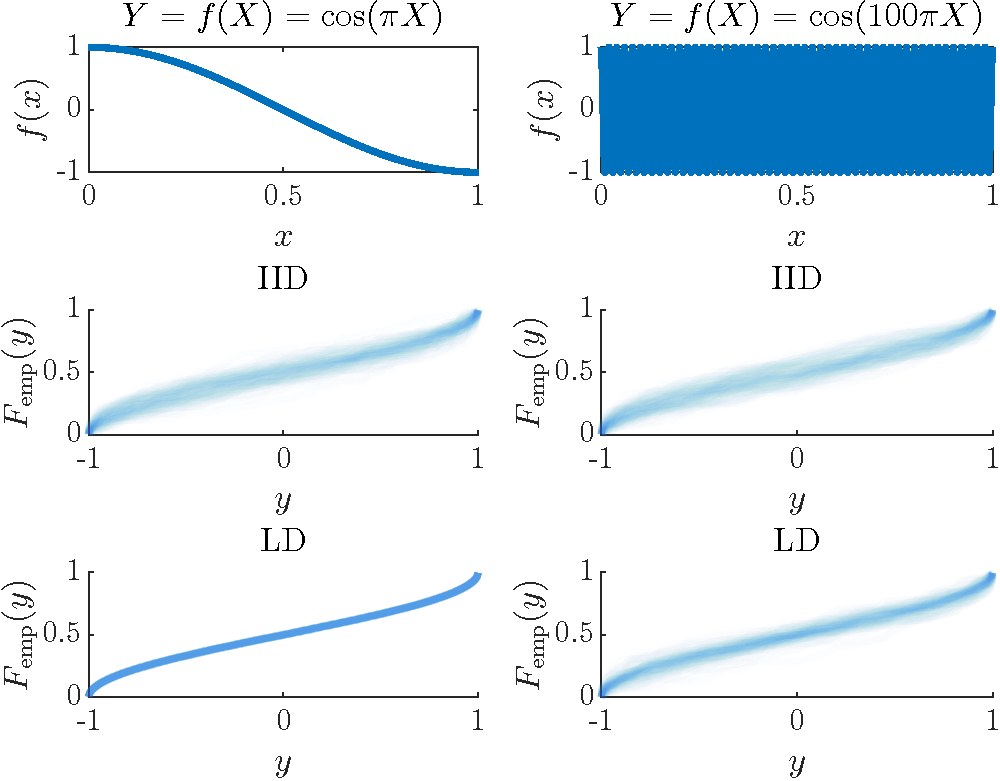
\includegraphics[width = 0.5\textwidth]{ProgramsImages/distribExperEG.pdf}
	\caption{Comparison of the empirical distribution functions of $Y = f(X)$ using $n=64$ IID and LD $X_i$ and for two definitions of $f$. The empirical distributions generated by LD points are closer to the true distribution than IID sampling. \vspace{-2ex}} \label{fig:empdistcomp}
\end{wrapfigure}

Although the distribution, $F$, is defined as an integral in \cref{eq:distdensquant}, the integrand as it stands, $\bbone_{(-\infty,y]}(f(\cdot))$, is insufficiently smooth for \QMC theory to apply directly, and thus there has been little developments on \LD sampling for such a setting (see \LimFour). Approximating the density (derivative of $F$) and quantile function, (inverse of $F$) are harder problems. Despite such theoretical challenges, \LD sequences show promise in approximating distributions, densities, and quantiles.  Consider two different definitions of $Y = f(X)$, $X \sim \calu[0,1]$ as shown in \cref{fig:empdistcomp}.  For both choices the distribution function of $Y$ is  $F: y \mapsto \sin^{-1}(y)/\pi + 1/2$.  \cref{fig:empdistcomp} displays $N = 100$ replications of the empirical distribution, $F_{\mathrm{emp}}$ based on $n=64$ \IID and \LD samples.  The \LD points provide better approximations of the distribution, and they provide better approximations for smoother $f$.

A recent study of \LD sequences for kernel density estimation \cite{AbdEtal21a} has demonstrated that in practice they outperform \IID sequences.  The authors also derive theoretical error bounds on this estimator for \LD sequences, but such bounds appear to be too loose. A tight quantification of uncertainty for density estimation is critical in our \UAV application, enabling sound design and control decisions. There has also been little work on investigating (and mitigating) the curse-of-dimensionality for density estimation with \LD sequences, a fundamental topic in \QMC \cite{dick2013high}. In \QMC, effective dimension is defined roughly as the number of coordinates of the input vector $\bX$ that make substantial contributions to $f(\bX)$. One expects that small effective dimension plays an important role in approximating  $\varrho$ with \LD sequences, just as it is in approximating  $\mu = \bbE[f(\bX)]$ with \LD sequences \cite{dick2013high}. This is crucial in our \UAV problem, where there are a broad range of design and control parameters for engine operation.

\subsubsection{Exploring the Effectiveness of LD Sequences.}[Year 1--3] The theory for using \LD sequences to estimate distributions, densities, and quantiles is in its infancy, which tempers our ambitions for these problems. Our first step will be to empirically compare the efficiency of \LD sequences to \IID sequences by inserting \LD sequences into standard algorithms that use \IID sequences, most likely some form of kernel smoothing \cite{WanJon95a}.  We will experimentally explore how to choose the band-width of kernel smoothing methods.  We will explore how the nominal dimension, the effective dimension, and the smoothness of $f$ influence the effectiveness of \LD sequences.  We will investigate its effectiveness in extensive experiments on the test function library \cite{VirLib17a}.

Based on  our computational experiments, we will derive data-driven algorithms that compute optimal bandwidth for smoothing and determine the sample size needed to satisfy the error criterion.  We will pursue the two approaches used for stopping criteria for computing $\mu$, namely i) analyzing the Fourier coefficients of $f$, and ii) assuming $f$ comes from a Gaussian process. We will demonstrate the effectiveness of such methods on our \UAV flight application.



\section{Broader Impacts}

% \cmtS{``Broader Impacts and Implementation''? We can then discuss \QMCPy as an open-source vessel for disseminating the proposed framework, geared towards the goal of scientific progress \& engineering advancement, etc.}

\subsection{Dissemination to the Broad Scientific Community.}
For the proposed suite of methods to become an integral tool for modern scientific discovery, scientists and engineers need to be convinced that our sampling paradigm can achieve confident and accurate estimates in a cost-efficient manner. This necessitates a \textit{strategic outreach} and \textit{targeted dissemination} of our methodologies to scientific communities who may not be familiar with the potential of \LD sampling for accelerating scientific discovery. We will achieve this via a \textit{multi-disciplinary} publication plan that targets a broad multi-disciplinary audience. We will publish in not only statistics, mathematics, and computer science journals, but also top subject-matter journals to make the proposed tools accessible to the scientific community. We will post all work as freely accessible papers on arXiv, with links to open source and well documented code on GitHub to allow for easier dissemination of our methods to end-users. We will also give talks, tutorials and workshops at prominent statistics, machine learning, and scientific conferences, educating different communities on promising developments on novel \LD methods for furthering scientific progress.

By broadening \QMC methods for tackling complex scientific and engineering problems, our project will naturally \emph{introduce new application areas} to the benefits of \LD sampling. The accessibility of state-of-the-art QMC methods in our outreach will spur on novel advancements in many scientific disciplines. We will focus specifically on four areas:

% This will lead to \emph{LD sampling being incorporated} into the software packages used by practitioners in those disciplines. This includes, e.g., PyMC3 \citep{salvatier2016probabilistic} and PyStan \citep{stan2017pystan}, which are popular Python packages for Bayesian statistical modeling and machine learning.

% A recent application of QMC for UQ is to compute the expectation of a functional of solution of a partial differential equation with random coefficients \cite{HerSch20a}. This has broad applications in engineering problems, e.g., fluid flow through a porous medium.
\subsubsection{Uncertainty Quantification (UQ).} UQ is the science of quantifying and managing uncertainty in computational and physical systems \cite{smartuq, Smi14a}. Since data are typically expensive for UQ, a key focus is the design of sampling points for experimentation. QMC can thus yield great computational savings for UQ (see \cite{HerSch20a} for a convincing application in fluid flows). PI \SM has ongoing multi-disciplinary collaborations on UQ in aerospace engineering \cite{li2017two,li2018uncertainty,chang2019kernel,yeh2018common,mak2018efficient,chang2021reduced}, nuclear physics \cite{ji2021graphical,ji2022multi,everett2021multisystem,everett2021phenomenological,cao2021determining, liyanage2022efficient,ehlers2022bayesian,kumar2022inclusive}, astrophysics \citep{mak2018maximum,zheng2021online,makinformation} and neuroscience \cite{wang2020uncertainty,wang2021sequential}, and we will introduce the benefits of \LD sampling for UQ in such disciplines.
\subsubsection{Machine Learning (ML).} Machine learning is a rapidly growing area with broad applications in science and engineering. Given the prevalent use of Monte Carlo in ML algorithms \cite{Bot2010,friedman2002stochastic,quiroz2018speeding}, \QMC will undoubtedly have a significant impact in this area (see \cite{Keller2013a} for a stunning application of \QMC in image rendering, and \cite{chen2019quasi} for an application of \QMC for learning PDEs). In addition to LD big data subsampling (\cref{sec:bigdata}), we will \textit{show the advantages of \QMC over \IID sampling in cutting-edge ML problems}, an area where both PIs have prior publication record \citep{mak2018support,makinformation,joseph2021supervised}.

\subsubsection{High Energy Physics.} Physicists have begun to recognize the advantages of \LD sampling for generating parton distributions \cite{CouEtal22a}.  We will continue our recent discussions with this group to explore how to best employ \LD sampling for a cost-efficient simulation of such problems. PI \SM has an extensive publication record in high energy physics (see Section \ref{sec:jetscape} and \cite{ji2021graphical,ji2022multi,everett2021multisystem,everett2021phenomenological,cao2021determining, liyanage2022efficient,ehlers2022bayesian,kumar2022inclusive}).

% \AGSNote{the article at https://arxiv.org/abs/1911.01612 is another example of QMC for ML where it learns PDEs by training a neural network with \LD samples.}
% \SMNote{need? fill in a few sentences.}
% \subsubsection{Probabilistic Numerics}: 
\subsubsection{Bayesian Methodology.} In addition to expensive posterior sampling (\cref{sec:bayes}), we will explore two Bayesian areas which can greatly benefit from QMC. The first is \hypertarget{PNlink}{probabilistic numerics} (\PN), which presumes the solution of a mathematical problem follows a prior random process. PI \FH with his former PhD student \JR developed a fast Bayesian cubature method \cite{RatHic19a} using lattice LD sampling. \hypertarget{BOlink}{Bayesian optimization} (\BO) aims to minimize a black-box objective function, where evaluations are optimized via an acquisition function in the form of a high-dimensional integral.  \MM illustrates the advantages of LD sampling for \BO \cite[qEI with \QMCPy]{QMCBlog}, and PI \SM has also worked in this area \cite{mak2019analysis,chen2019hierarchical}. We will demonstrate the \emph{efficacy of LD sampling} in \BO and \PN.

% We will publish our theoretical and practical work in a variety of mathematics, statistics, and computer science journals and conference proceedings. We will present our work at conferences targeting theoreticians and practitioners.  We will offer tutorials.  Students will present at conferences and during group meetings, as part of their education. \cmtS{expand and discuss cross-disciplinary dissemination to the broad scientific community? some sample writing below from another proposal}

% \subsubsection*{}

\subsection{QMCPy as a Proving Ground.} \label{sec:provingground} 
As mentioned in \cref{sec:lowdiscrep,sec:stopcrit}, \FH, \YD, \SCTC, \AS, \MM, \JR, \PR, and collaborators have created the open source Python QMC library \QMCPy \cite{QMCPy2020a}.  \QMCPy has a clear architecture and consistent user interface. It includes \LD sequences,  variable transformations, and stopping rules.  \QMCPy is hosted on a GitHub repository 
%\cmtS{should we provide link?} it is in the reference
with documentation, a suite of doctests and unit tests, Jupyter notebook demos, and an issues board. With this architecture, \QMCPy will serve as an ideal vessel for bridging our suite of methods (and state-of-the-art \QMC algorithms) to the scientific community, thus addressing \LimFive.

\QMCPy will continue to grow and \emph{stand in the breach} between research code from individual groups and large-scale software packages.  Research groups need to compare their new ideas with the best available. Developers for \LD generators need to test them on a variety of use cases and as key components of \QMC algorithms.  Those with new QMC algorithms need to test them with the best generators. We will connect \QMCPy to other libraries in \cref{sec:lowdiscrep}, taking advantage of what they offer in \QMCPy and pushing our more established developments into them.  We recently collaborated with Uncertainty Quantification and Model Bridge (UM-Bridge) \cite{umbridge} to make \QMCPy compatible with UM-Bridge. A recent gathering at an international \QMC conference initiated by \FH raised the need to standardize formats for \LD generators to allow them to be shared across software libraries.  We will initiatives that promote same look-and-feel across \QMC software.

%%%%%%%%%%%%%%%%%%%%%%%%%%%%%%%%%%%%%%%%%%%%%%%%%
\subsection{Promoting Proper QMC Practice and Code.} \label{sec:goodpractice}
%%%%%%%%%%%%%%%%%%%%%%%%%%%%%%%%%%%%%%%%%%%%%%%%%
\QMCPy---software, documentation, academic articles, and conference presentations---will \emph{showcase the right way} to do \LD sampling.  As an example, the adoption of \PyTorch into \QMCPy and the tutorial given by \FH at MCQMC 2020 \cite{MCQMC2020QMCPyTut, ChoEtal22a} prompted a vigorous discussion on the \PyTorch issues site \cite{PyTorchFirstPt2020a} that migrated to the \SciPy issues site \cite{scipySobol2020a}.  \AO, \FH, and other QMC researchers convinced the developers to not omit the first Sobol' point, but to randomize by default.  Keeping the first point preserves the net property of the first $2^m$ Sobol' points and randomization can speed up convergence~\cite{owen2020dropping}. In these discussions, it was pointed out that UQLab \cite{UQLab2014}, OpenTurns \cite{OpenTURNS}, and other packages routinely drop the first Sobol' point, a bad but understandable practice.  The arguments we provided to \PyTorch and \SciPy developers addressed their concerns.  We expect this project to produce fruitful discussions between QMC practitioners, which will promote better practice.

Having the eyes of the QMC community on \QMCPy will more \emph{quickly uncover and eradicate bugs}.  \FH found  that randomized \PyTorch Sobol' points fell on the boundaries of $[0,1]^d$, when they never should \cite{PyTorchFirstPt2020a} This was due to a lack of double precision, as discovered by \MM.  \LlAJR found that the Sobol' scrambling in \MATLAB was incorrect.  This was rectified in R2017a.  This highlights how having a larger community using a software library leads to higher quality code.



% Educating and Mentoring Cross-Disciplinary Computational Researchers
\subsection{Training the Next Generation of {\em Science-Based} Computational Researchers.}

There is a critical need for individuals who have the computational and mathematical tools to adeptly work in modern \textit{scientific} teams, geared towards pushing forward the frontier of scientific knowledge and engineering through improved science-based data science tools. Students involved in this project will be given a \textit{multidisciplinary} background in science-based data science, and will learn relevant methods in statistics, mathematics and computer science. This will serve them well in transitioning to not just academic research teams but also government and industry positions.
% Traditional data science has been largely driven by \textit{purely} predictive problems that arise in the tech industry, while \textit{science-based} data science is focused on building realistic models and obtaining interpretable insights from sophisticated virtual and real-world experiments.

Computational mathematics and statistics require the use of others' code, hopefully in the form of well-developed software packages. New scholars also need to be trained not only on how to use such packages, but how to contribute to them as well. Students supported by this project will learn to write clean, efficient code that fits package architecture, is documented, and passes doctests. Students will learn about repositories and software engineering tools, which will prepare them well for academic and/or industry opportunities.

% Some will learn how to combine code from different packages and even different languages.
 % just like Beamer became second nature to many a generation ago, and \LaTeX\ two generations ago
 
\subsection{Incorporating Diversity, Equity and Inclusion} As with past projects, in seeking students, we will give preference to underrepresented minorities, women, and students from colleges where research experiences are rare.  As noted in \cref{sec:PreviousFred,sec:jetscape}, we have had a strong track record of mentoring students from \textit{diverse} backgrounds and experiences. Five of \FH's fifteen students who earned PhDs are women, three of whom are academics. \FH supervised an African-American student, \CH, in the Summer Undergraduate Research Experience (SURE) program at Illinois Tech, which provides research opportunities particularly for underrepresented groups. \CH is now a PhD student at Illinois Tech.
Two of \SM's seven current PhD students are women, and five of \SM's ten undergraduate thesis advisees are women. Many of our undergraduates have enrolled in graduate programs. \SM is on the leadership board of the IMS New Researchers Group, which aims to provide career development opportunities for young statisticians, particularly those from underrepresented backgrounds and institutions.
 % will keep collaborating with SURE to involve more underrepresented students in the research group and encourage them to pursue an advanced degree

We will leverage these connections to further promote diversity and inclusion, providing students from underrepresented backgrounds and institutions with ample research training and opportunities. The senior personnel on this project include two women (\SCTC and \YD) and one early-career scholar (\SM).  Our senior personnel and collaborators include folks with diverse technical expertise, institutions and backgrounds. The students that we mentor in this project will also learn and benefit from thinking from these diverse perspectives.

% % \subsection*{}
% \subsection{Expanding the Scope of QMC Applications} \label{sec:scopeapplication} 





\section{Results from Prior NSF Support} \label{sec:prior_work}

% \cmtS{should we shorten slightly here for page limit?}

\subsection{NSF-DMS-1522687, \emph{Stable, Efficient, Adaptive Algorithms for
		Approximation and Integration},
	\$270,000, August 2015 -- July 2018.} \label{sec:PreviousFred}
%%%%%%%%%%%%%%%%%%%%%%%%%%%%%%%%%%%%%%%%%%%%%%%%%%%%%%%%%%%%%%%%%%%%%%%%%%%%%%%%%%%
Fred Hickernell (\FH, PI) and Gregory E. Fasshauer (\GEF, co-PI) led this project, and \SCTC contributed as senior personnel. Other contributors were \FH's research students {\YD} (PhD 2015), \LJ (PhD 2016),
\LlAJR (PhD 2016), \hypertarget{DLlink}{Da Li} (\DL, MS 2016), \hypertarget{JLlink}{Jiazhen Liu} (\JL, MS 2018), JR (PhD 2019), \hypertarget{XTlink}{Xin Tong} (\XT, MS 2014, PhD 2020 at the University of Illinois at Chicago), \hypertarget{KZlink}{Kan Zhang} (\KZ, PhD student), \hypertarget{YZlink}{Yizhi Zhang} (\YZ, PhD 2018), and \hypertarget{XZlink}{Xuan Zhou} (\XZ, PhD 2015).  Articles, theses,
software, and preprints supported in
part by this
grant
include
\cite{ala_augmented_2017,
	ChoEtal17a,
	ChoEtal21a,
	Din15a,
	DinHic20a,
	GilEtal16a,
	Hic17a,
	HicJag18b,
	HicJim16a,
	HicEtal18a,
	HicEtal17a,
	HicKriWoz19a,
	RatHic19a,
	GilJim16b,
	JimHic16a,
	JohFasHic18a,
	Li16a,
	Liu17a,
	MarEtal18a,
	mccourt_stable_2017,
	MCCEtal19a,
	mishra_hybrid_2018,
	MisEtal19a,
	rashidinia_stable_2016,
	rashidinia_stable_2018,
	Zha18a,
	Zha17a,
	Zho15a,
	ZhoHic15a}.

%%%%%%%%%%%%%%%%%%%%%%%%%%%%%%%%%%%%%%%%%%%%%%%%%%%%%%%%%%%%%%%%%%%%%%%%%%%%%%%%%%%
\subsubsection{Intellectual Merit from Prior NSF Support.}
\label{previousmeritsubsec}
%%%%%%%%%%%%%%%%%%%%%%%%%%%%%%%%%%%%%%%%%%%%%%%%%%%%%%%%%%%%%%%%%%%%%%%%%%%%%%%%%%%

\FH, \SCTC, \YD, \LlAJR, \DL, \JR, \XT, \YZ,   and  developed several adaptive algorithms for univariate integration, function approximation, and optimization \cite{ChoEtal17a,HicEtal14b,  Din15a, Ton14a, Zha18a}, multivariate integration \cite{HicJim16a,HicEtal17a,JimHic16a}, and multivariate function approximation for Banach spaces, $\calf$, defined by series representations \cite{DinHic20a,DinEtal20a}.  

%%%%%%%%%%%%%%%%%%%%%%%%%%%%%%%%%%%%%%%%%%%%%%%%%%%%%%%%%%%%%%%%%%%%%%%%%%%%%%%%%%%
\subsubsection{Broader Impacts from Prior NSF Support.} \label{prevBIsect}
%%%%%%%%%%%%%%%%%%%%%%%%%%%%%%%%%%%%%%%%%%%%%%%%%%%%%%%%%%%%%%%%%%%%%%%%%%%%%%%%%%%
Publications by \GEF, \FH,  \SCTC, students, and collaborators are listed above.  We have spoken at many applied mathematics, statistics,
and computational science conferences and given colloquium/seminar talks to mathematics and
statistics departments.  \FH co-organized the
2016 Spring Research
Conference, gave an invited tutorial
at MCQMC 2016, was a program leader for the SAMSI 2017--18 Quasi-Monte Carlo (QMC) Program, and received the 2016 Joseph F.\ Traub Prize for Achievement in Information-Based Complexity.  Our adaptive algorithmshave been been implemented in
\GAIL \cite{ChoEtal21a}, which has been used in the graduate Monte Carlo at Illinois Tech. The PIs mentored a number of
research students;  female students include \YD, \LJ, \JL, \XT, and Xiaoyang Zhao (MS 2017).


% \FJHNote{Simon, do you need to put two prior support or just one?} \cmtS{commented other one for now - not sure if required for both}
\subsection{NSF CSSI Frameworks 2004571 (Subaward WSU20076). \textit{X-Ion Collisions with a Statistically and Computationally Advanced Program Envelope (X-SCAPE),} \$696,442, July 2020 -- June 2024.} \label{sec:jetscape}

High-energy colliders study the interaction between subatomic particles and environments produced in the collision of protons with protons and with nuclei. This requires an elaborate theoretical, statistical and computational framework. The X-SCAPE (\hypertarget{JetscapeLink}{JETSCAPE}) collaboration is a multi-disciplinary team of physicists, computer scientists, and statisticians, who are engaged in the construction of such a framework. \SM is a Duke co-PI in this 
ongoing project, and is responsible for leading statistical and ML developments.

\subsubsection{Intellectual Merit from Prior NSF Support.}

The JETSCAPE collaboration has developed the first open-source simulation framework for the high energy sector of heavy-ion collisions and a Bayesian framework to rigorously compare event generators with experimental data. This has resulted in numerous publications in top physics journals and conferences \cite{cao2017multistage,kumar2019jetscape,everett2021multisystem,everett2021phenomenological,everett2022role,kumar2022inclusive,ehlers2022bayesian,cao2021determining,soltz2018bayesian,tachibana2018jet,kauder2019jetscape,park2019multi} and top statistical / ML journals and conferences \citep{chen2022adaptive,wang2021sequential,zheng2021online,mak2021tsec,yuchi2021bayesian,huang2022population,chen2020function,zhang2022gaussian}.

\subsubsection{Broader Impacts from Prior NSF Support.}
The primary broader impacts of the X-SCAPE collaboration have been in the training of its graduate students and postdocs, through regular meetings, collaboration gatherings, and joint projects. The collaboration also influences the training of the wider US nuclear physics workforce through its annual winter school and workshops. \SM is supporting several students on this project, including two female PhD students and two female undergraduates. \SM is co-organizing the 2023 Spring Research Conference, and received the 2022 Rosenbluth-Blackwell Award for exceptional career achievements by a junior Bayesian researcher.

% \subsection{NSF DMS 2210729 \emph{SCience-INtegrated Predictive modeLing (SCINPL): a novel framework for scalable and interpretable predictive scientific
% modeling},
% 	\$200,000, August 2022 -- July 2025}\label{sec:scinpl}

%  \subsubsection{Intellectual Merit from Prior NSF Support}
% \SM is the PI for this ongoing project on developing statistical methods for integrating scientific knowledge as prior beliefs within Bayesian predictive models. In scientific computing problems with limited training data, this suite of methods aims to provide improved predictive performance with reduced uncertainty, thus enabling interpretable and cost-efficient scientific discovery. Manuscripts of all research developments are posted on arXiv, and have already been downloaded and cited many times.

% \subsubsection{Broader Impacts from Prior NSF Support}
% Several students are currently supported by this project, and are actively involved in a broad range of scientific collaborations with nuclear physicists, aerospace engineers, and material scientists. This project has led to many publications \citep{sung2022stacking, ji2021graphical, ji2022multi, mak2021tsec, chen2022adaptive, yuchi2021bayesian, zhang2022gaussian,zheng2021online}, including in top statistics and domain science journals.

% \subsection{Co-PI Yuhan Ding has no prior NSF support to report}

\section{Strengths of This Team and Collaboration Plan}
Our team combines senior personnel with diverse backgrounds, career stages, and institutions. We will have regular meetings to share progress and collaborate on papers and software. These will be held both at our own institutions and via video conference between institutions.

% \cmtS{May need further thought on DEI, seems to be increasingly important for grants nowadays.}

% We will grow \QMCPy into what it should become while providing new theories and methodologies to underpin our new algorithms. The leads and team members for each topic are identified above, along with the years for each task. 

\subsection{Senior Personnel.}
\FH has been the lead PI on the GAIL \cite{ChoEtal21a} \MATLAB software project that contains many of the stopping criteria in \QMCPy. His expertise is in the numerical analysis of QMC and other multivariate problems as well as theoretically justified adaptive numerical algorithms.  As a former editorial board member for major computational mathematics journals, a Fellow of the Institute of Mathematical Statistics, and a co-leader of SAMSI's program on QMC in 2017-18, \FH understands the interface between computational mathematics and statistics.

\SM is an Assistant Professor at Duke, specializing in Bayesian computation, big data analytics, and computer experiments. As an Associate Editor for \textit{Technometrics} (a top engineering statistics journal) and \textit{Data Science in Science}, and the recipient of major awards from the American Statistical Association and the International Society of Bayesian Analysis, \SM provides expertise on statistical / ML methods and applications. \SM will lead the activities at Duke and oversee the proposed efforts on Bayesian sampling and big data subsampling.

% He also has experience in software library development, having authored four \textsc{R} packages \cite{support,minimaxdesign,cmenet,atmopt} on the Comprehensive R Archive Network (CRAN).

\YD is an associate teaching professor at Illinois Tech, who teaches Monte Carlo methods in finance and programming for data analytic. She is experienced in the theory and implementation of QMC and adaptive algorithms, and is one of the main developers of the GAIL project.

% She is familiar with QMC methods and has started using  \QMCPy in her course.

\SCTC serves as a Principal Data Scientist at SAS in the financial risk group.  She is a research associate professor at Illinois Tech.  \SCTC has co-led the GAIL and \QMCPy projects and is an expert in best engineering practices for numerical software.  She is a co-winner of the 2011 Society for Industrial and Applied Mathematics Activity Group on Linear Algebra best paper prize.


\subsection{Students.}  \AS began his PhD in applied mathematics at Illinois Tech in Fall 2021 after completing a dual BS/MS degree at Illinois Tech and doing a large majority of the coding of \QMCPy to date. \CH is an African American Illinois Tech PhD student who began in Fall 2022.  \IJi, \TT, \JM and \KL are Statistical Science PhD students at Duke University, working on theory and methods for computer experiments, uncertainty quantification, Bayesian computation and big data analytics, with applications to physics and engineering. PhD students supported by this project will work with the senior personnel to tackle major theoretical and methodological challenges.  Undergraduate students will focus on new features that can be implemented mostly over the course of a summer.  They will be mentored by senior personnel and PhD students. 

\subsection{Collaborators.}
The responsibilities of these unpaid collaborators will be to discuss research ideas of common interest, involve their research groups as appropriate, and publish significant results.  We have identifed above some of the projects that they may be involved in.
\MM convinced his company to fund the early development of \QMCPy.  He wanted to spread the advantages of \LD sampling to the tech industry. \MM will advise us on the continued development of \QMCPy, and continue to help us spread the word among his network in the machine learning community.
\AO has engaged with the PIs in conversations about \QMC for many years and is particularly an expert in randomized \QMC.  \AO has taken a keen interest in \QMCPy and used it in his own research. 
\PR has wide experience in multi-level methods and uncertainty quantifciation applications of QMC.
\CO is an expert in \PN.  He will provide expertise on the use of Stein discrepancy points and also  Bayesian numerics for stopping criteria for \QMC methods.

%\end{document}

\newpage
\clearpage
%\pagenumbering{arabic}
\setcounter{page}{1}
%\renewcommand{\thepage}{D-\arabic{page}}

\bibliographystyle{spbasic}


{\renewcommand\addcontentsline[3]{}
\renewcommand{\refname}{{\Large\textbf{References Cited}}}                   %%
\renewcommand{\bibliofont}{\normalsize}

\bibliography{FJH23,FJHown23,simon,choi}
\end{document}

%%%%%%%%%%QMCPy%%%%%%%%%%%%%%%



 \QMCPy may be installed using \pyinline{pip} and imported via \pyinline{from qmcpy import *}.

 
\subsubsection*{\textup{\pyinline{DiscreteDistribution} and \pyinline{TrueMeasure}}} \LD sequences are constructed by creating the object and then generating points.  The code below produces the center panel of \cref{fig:iid_vs_ld}.
% \vspace{-0.7cm}
\begin{pythoncode}
lattice = qmcpy.Lattice(dimension = 2) #define a discrete \LD distribution
points = lattice.gen_samples(n = 64)   #construct points
\end{pythoncode}
% \vspace{-0.2cm}
\indent \LD generators provide points designed to mimic the distribution $\calu[0,1]^d$.  \QMCPy also has \pyinline{Sobol} \cite{DicPil10a} and \pyinline{Halton} \cite{Hal60} \LD generators whose syntax are comparable. \QMCPy  has standard uniform and normal pseudorandom generators adopted from \pyinline{numpy} for comparison purposes.  

\begin{wrapfigure}{r}{0.50\textwidth}
	\centering
	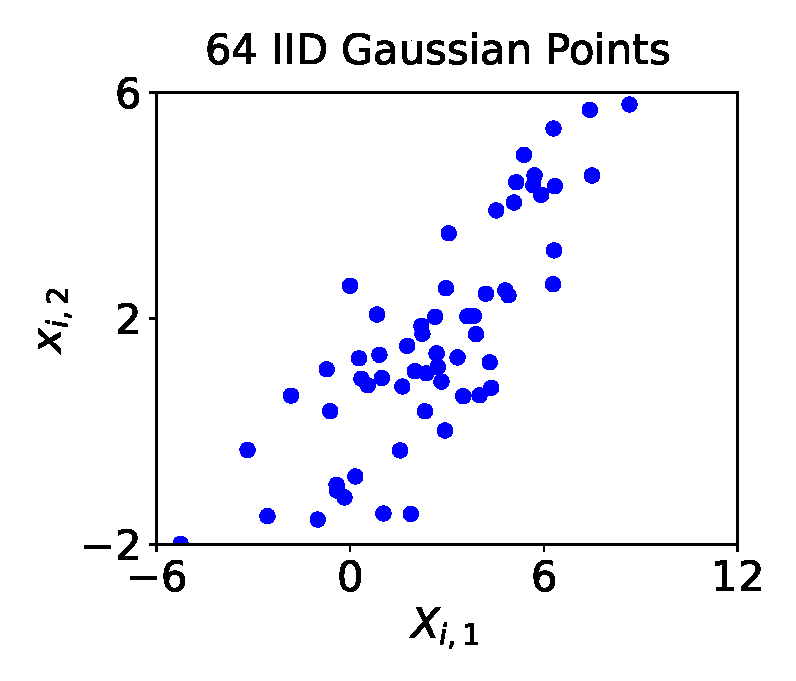
\includegraphics[height = 3.0cm]{ProgramsImages/Gauss_IID.eps}
	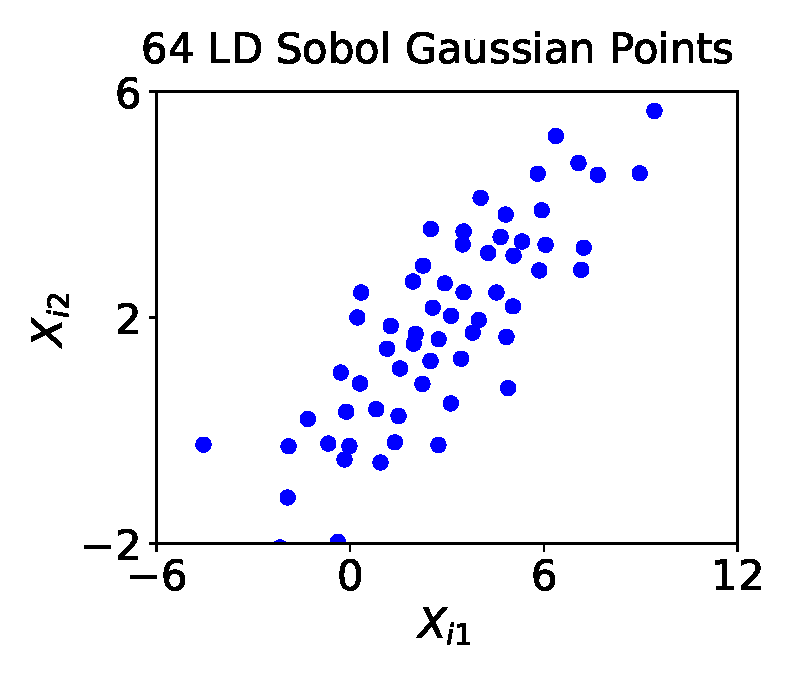
\includegraphics[height = 3.0cm]{ProgramsImages/Gauss_Sobol.eps}
	\caption{IID Gaussian (left) and Sobol'  points transformed to mimic a Gaussian distribution (right).  The \LD points better represent the Gaussian distribution than the \IID points. \label{fig:ld_Gauss}}
	\vspace{-0.3cm}
\end{wrapfigure}

One may generate additional points while reusing the original ones.   \QMCPy \LD generators are randomized by default to ensure that no points lie on the boundary of the unit cube and to improve the order of convergence of $\hmu_n$ to $\mu$ \cite{Owe97}. The \pyinline{TrueMeasure} class automates the transformation required to construct good points that mimic distributions other than standard uniform.  The  inverse  distribution is often used.  \cref{fig:ld_Gauss} displays  \IID and Sobol' points  transformed to mimic a multivariate  Gaussian distribution.
%with mean $\begin{pmatrix} 3 \\ 2 \end{pmatrix}$ and covariance matrix $\begin{pmatrix} 9 & 5 \\ 5 & 4 \end{pmatrix}$.  
\begin{pythoncode}
gaussian_ld = qmcpy.Gaussian(qmcpy.Lattice(2), mean = [3,2], covariance = [[9,5],[5,4]])  #specify the distribution parameters
points = gaussian_ld.gen_samples(n = 64)  #construct points
\end{pythoncode}

%%%%%%%%%%%%%%%%%%%%%%%%%%%%%%%%%%%%%%%%%%%%%%%%%
\subsubsection*{\textup{\pyinline{Integrand} and \pyinline{StoppingCriterion}}}
%%%%%%%%%%%%%%%%%%%%%%%%%%%%%%%%%%%%%%%%%%%%%%%%%
One must specify the integrand to compute expectations and multivariate integrals as described in \eqref{eq:mean}.   The original form of the problem may not be convenient for computation.  For example, the Keister integral in \eqref{eq:Keister} can be thought of as an integral of $g$ with respect to the Gaussian distribution with zero mean and covariance $\mI/2$:
\begin{multline} \label{eq:KeisterAlt}
\mu = \int_{\reals^d} \underbrace{\pi^{d/2} \cos( \norm[2]{\bt})}_{g(\bt)}  \, \underbrace{\pi^{-d/2}\exp(-\norm[2]{\bt}^2)\, \dif \bt}_{\caln(\bzero, \mI/2)}
= \int_{\reals^d} \underbrace{\cos( \norm[2]{\bt}) \exp(-\norm[2]{\bt}^2)}_{h(\bt)}  \, \underbrace{\dif \bt}_{\text{Lebesgue}} \\
=   \int_{[0,1]^d} f(\bx) \, \dif \bx \qquad \text{for an appropriate transformation } \bt = \bT(\bx).
\end{multline}
Alternatively, $\mu$ can be thought of as an integral of $h$ with respect to Lebesgue measure.  \QMCPy can compute the integral either way.

The first way begins by constructing the Gaussian transformed \LD \pyinline{TrueMeasure} instance \pyinline{gs} as described in the previous section.  Next, one defines the function $g$ as in \eqref{eq:KeisterAlt} above.   \pyinline{CustomFun}  constructs an $f$ for which the integral, $\mu$, can be written in terms of the uniform distribution, which the \LD sequence mimics.   \pyinline{CustomFun} automatically constructs the transformation $\bT$ in \eqref{eq:KeisterAlt}.
\begin{pythoncode}
gs = qmcpy.Gaussian(qmcpy.Sobol(5), covariance = 1/2)    #choose the Gaussian distribution
def g(t):  #your desired integrand, calculations must be vectorized
	d = t.shape[1]
	g_val = np.pi**(d/2) * np.cos(np.sqrt((t**2).sum(1)))
	return g_val  #size n vector
f = qmcpy.CustomFun(gs, custom_fun = g)
sc = qmcpy.CubQMCSobolG(f, abs_tol = 1e-3)   #stopping criterion must match  points
solution, data = sc.integrate()
\end{pythoncode}

The final stage of the computation requires the construction of a \pyinline{StoppingCriterion} instance, \pyinline{sc}.  The one here is due to PI \FH and \hypertarget{LlAJRlink}{Llu\'is Antoni Jim\'enez Rugama} (\LlAJR) \cite{HicJim16a} and is based on Walsh transformations of the sampled integrand data.  Invoking the \pyinline{integrate} method of \pyinline{sc} yields $\hmu_n$ satisfying error criterion \eqref{eq:error_crit} and a data object containing summary results.

Another way to compute the Keister integral \eqref{eq:KeisterAlt} is to think of it as an integral with respect to the Lebesgue measure.  Again \pyinline{CustomFun} selects a default variable transformation or sampling measure.  The answer from QMCPy is the same as the first way, but this second way takes twice the time.  The choice of variable transformation, $\bT$, that defines $f$ from the original integrand is equivalent to importance sampling.  Automatic and adaptive importance sampling requires further research (see Sec. 3.3).